% !TeX spellcheck = de_DE
\documentclass[a4paper, twoside, 12pt, openright]{memoir}
\usepackage[T1]{fontenc}
\usepackage[margin=2cm, bindingoffset=10mm, includeheadfoot, headheight=14.7pt]{geometry}
\usepackage[british, ngerman]{babel}
\usepackage[hyperref=true]{acro}
\usepackage[backend=biber, style=ieee]{biblatex}
\usepackage[final]{minted}
\usepackage{fancyhdr, 
	graphicx,
	datetime2,
	fontspec,
	float,
	hologo,
	csquotes,
	longtable,
	pdfpages,
	multirow,
	tabulary,
	amsmath,
	blindtext}
\usepackage[protrusion=true,final]{microtype}
\usepackage[final]{hyperref}
\usepackage[all]{hypcap}

%\overfullrule=1mm

\addbibresource{sources.bib}
\acsetup{
	first-style = short
}

\DeclareAcronym{dotnet}{
	short = Net\-Fx,
	alt = dot\-Net\-Fx, 
	long = .NET-Rahmenwerk,
	foreign = .NET-Framework,
	foreign-lang = british,
}

\DeclareAcronym{rpi}{
	short = RPi,
	alt = Ras\-Pi,
	long = Raspberry Pi
}

\DeclareAcronym{rtsp}{
	short = RTSP,
	long = Real Time Streaming Protocol
}

\DeclareAcronym{sdk}{
	short = SDK,
	long = Software Development Kit
}

\DeclareAcronym{ndk}{
	short = NDK,
	long = Native Development Kit
}

\DeclareAcronym{fi}{
	short = FI,
	long = Fachspezifische Softwaretechnik
}

\DeclareAcronym{css}{
	short = CSS,
	long = Cascading Style Sheets
}

\DeclareAcronym{rtp}{
	short = RTP,
	long = Real-time Transport Protocol
}

\DeclareAcronym{rtcp}{
	short = RTCP,
	long = Real-Time Control Protocol
}

\DeclareAcronym{vod}{
	short = VOD,
	long = Video on Demand
}

\DeclareAcronym{apk}{
	short = APK,
	long = Android Package
}

\DeclareAcronym{eagle}{
	short = EAGLE,
	long = Einfach Anzuwendender Grafischer Layout-Editor,
	%foreign = Easily Applicable Graphical Layout Editor
}

\DeclareAcronym{pcb}{
	short = PCB,
	long = Leiterplatte,
	foreign = Printed Circuit Board
}

\DeclareAcronym{smd}{
	short = SMD,
	long = oberflächenmontiertes Bauelement,
	foreign = Surface-mounted Device
}

\DeclareAcronym{ic}{
	short = IC,
	long = integrierte Schaltung,
	foreign = Integrated Circuit
}

\DeclareAcronym{uwp}{
	short = UWP,
	long = universelle Windows-Plattform,
	foreign = Universal Windows Platform
}

\DeclareAcronym{tht}{
	short = THT,
	long = Through-Hole Technology
}

\DeclareAcronym{clr}{
	short = CLR,
	long = Common Language Runtime
}

\DeclareAcronym{cil}{
	short = CIL,
	long = Common Interface Language
}

\DeclareAcronym{http}{
	short = HTTP,
	long = Hyper-Text Transport Protocol
}

\DeclareAcronym{mvvm}{
	short = MVVM,
	long = Model-view-viewmodel
}
%TeX distance tweaking
\emergencystretch=1em%
\makeatletter
  \renewcommand{\@pnumwidth}{3em}
  \renewcommand{\@tocrmarg}{4em}
\makeatother

%global package setups
\hypersetup{
	linktoc=all,
	colorlinks=false,
	linkcolor=blue
}

\setminted[csharp]{
	numbers=both, 
	breaklines=true,
	% breakbefore=;:\=\,.,
	breakafter=;:\=\,.
}
\setminted[xml]{
	numbers=both,
	breaklines=true,
	%breakbefore=;:\=\,.,
	breakafter=;:\=\,.
}
\setminted[text]{
	numbers=both,
	breaklines=true,
	%breakbefore=;:\=\,.,
	breakafter=;:\=\,.
}
\setminted[arduino]{
	numbers=both,
	breaklines=true,
	%breakbefore=;:\=\,.,
	breakafter=;:\=\,.
}

% pagestyles ------------------------------------------------------------------
\fancypagestyle{normalpage}{
	\fancyhf{} %clear header and footer
	\rhead[\leftmark]{\thepage}
	\lhead[\thepage]{\rightmark}
	\cfoot{\authorName}
	\renewcommand{\headrulewidth}{0.4pt}
	\renewcommand{\footrulewidth}{0.4pt}
}
\aliaspagestyle{chapter}{normalpage}

\fancypagestyle{abstractpage}{
	\fancyhf{} %clear header and footer
	\rhead[]{\thepage}
	\lhead[\thepage]{}
	\cfoot{\authorName}
	\renewcommand{\headrulewidth}{0.4pt}
	\renewcommand{\footrulewidth}{0.4pt}
}
\aliaspagestyle{part}{abstractpage}

\fancypagestyle{titlepage}{
	\fancyhf{} %clear header and footer
	\fancyhead[c]{\includegraphics[width=\linewidth]{images/HTL_Header}}
	\cfoot{\authorName}
	\renewcommand{\headrulewidth}{0.4pt}
	\renewcommand{\footrulewidth}{0.4pt}
}
\aliaspagestyle{titlingpage}{titlepage}

% memoir configuration ------------------------------------------------------
\chapterstyle{section}
\setsecnumdepth{subsubsection}
\settocdepth{subsection}

% custom commands -----------------------------------------------------------
\newcommand{\blankpage}{
	\newpage
	\null
	\thispagestyle{empty}
	\newpage
}
\newcommand{\MarioPrantl}{DI(FH) Mario Prantl}
\newcommand{\AndreasGrain}{Andreas Grain}
\newcommand{\MatthiasMair}{Matthias Mair}
\newcommand{\authorName}{\AndreasGrain\ / \MatthiasMair}
\newcommand{\crossref}[1]{\emph{\ref{#1} \nameref{#1}}}
\newcommand{\wip}{{\color{red}Nachfolgender Teil ist noch in Bearbeitung durch \authorName}}
\newcommand{\tOmega}{Ω}
\newcommand{\tdelta}{Δ}

% text formatting ----------------------------------------------------------
%\setlength{\parindent}{0pt}% Remove paragraph indentation
\setlength{\parskip}{8pt}% Add space after paragraph
\setmainfont{Arial}
\renewcommand{\footnotesize}{\scriptsize}

\setlength{\beforechapskip}{0pt}
\setlength{\afterchapskip}{20pt}
% Document start -----------------------------------------------------------
\begin{document}
\pagestyle{normalpage}

\frontmatter
\begin{titlingpage}
	\newgeometry{margin=2cm, bindingoffset=5mm, includeheadfoot, headheight=54pt}
\begin{center}
	\vspace*{2cm}
	\Huge\textbf{Diplomarbeit}\\
	\vspace*{2cm}
	\huge Bidirektionale Videosprechanlage\\
	\vspace*{0.5cm}
	\normalsize Erweiterung einer RaspberryPi basierten Videogegensprechanlage\\
	\vspace*{1.5cm}
	\textbf{Höhere Technische Bundeslehr- und Versuchsanstalt Anichstraße}\\
	\vspace*{0.5cm}
	\rule{0.75\linewidth}{0.4pt}\\
	\vspace*{0.5cm}
	Abteilung Elektrotechnik\\
	\vspace*{1cm}
	\begin{minipage}{0.425\linewidth}
		\begin{flushleft}
			Ausgeführt im Schuljahr 2019/20 von:\bigskip\\
			Andreas Grain 5AHET (HV)\\
			Matthias Mair 5AHET\\
		\end{flushleft}
	\end{minipage}
	\begin{minipage}{0.425\linewidth}
		\begin{flushright}
			Betreuer:\bigskip\\
			DI(FH) Mario Prantl\\
		\end{flushright}
	\end{minipage}
\end{center}
\vspace*{1cm}
%\hspace*{0.15\linewidth}Projektpartner: keine
\vfill
Innsbruck, am \today
\vspace*{1cm}
\hrule
\vspace*{1cm}
\begin{minipage}{0.49\linewidth}
	\begin{flushleft}
		Abgabevermerk:\\
		Datum:
	\end{flushleft}
\end{minipage}
\begin{minipage}{0.49\linewidth}
	\begin{flushleft}
		Betreuer:
	\end{flushleft}
\end{minipage}\\
\restoregeometry
\end{titlingpage}

\OnehalfSpacing

\chapter{Erklärungen}
\section{Eidesstattliche Erklärung}
Wir erklären an Eides statt, dass wir die vorliegende Diplomarbeit selbständig und ohne fremde Hilfe verfasst, andere als die angegebenen Quellen und Hilfsmittel nicht benutzt und die den benutzten Quellen wörtlich und inhaltlich entnommenen Stellen als solche erkenntlich gemacht haben.
\vspace*{1.5cm}
\begin{center}
	\hrule
	\vspace*{0.2cm}
	Ort, Datum\hspace*{0.4\linewidth}\AndreasGrain\\
	\vspace*{1.5cm}
	\hrule
	\vspace*{0.2cm}
	Ort, Datum\hspace*{0.4\linewidth}\MatthiasMair
\end{center}
\vspace*{1.5cm}

\section{Gender-Erklärung}
Aus Gründen der besseren Lesbarkeit wird in dieser Diplomarbeit die Sprachform des generischen Maskulinums angewendet.
Es wird an dieser Stelle darauf hingewiesen, dass die ausschließliche Verwendung der männlichen Form geschlechtsunabhängig zu verstehen ist.
\cleartoverso

\SingleSpacing
\tableofcontents
\OnehalfSpacing
%\cleartoverso

\chapter{Kurzfassung/Abstract}
Die vorliegende Diplomarbeit beschäftigt sich mit der Erweiterung einer \ac{rpi}-basierten Videosprechanlage um eine Smartphone-Applikation, sowie der grundlegenden Überarbeitung der Stations-Hardware.
Zusätzlich soll ein Linux-basierter, aus dem Internet erreichbarer Server zum Verteilen der Video-Streams eingerichtet werden.
%Für die Entwicklung der Smartphone-App wird das Xamarin-Framework herangezogen, sodass die Applikation sowohl auf Android-, als auch iOS-Geräten lauffähig ist.
\par
Dieses Projekt basiert auf einer früheren Diplomarbeit von Sebastian Wagner und Tobias Pfluger an der HTL Anichstraße aus dem Jahr 2017/18, welche ein voll funktionsfähiges Videosprechanlagensystem hervorbrachte.
Jedoch wurde damals die Hardware-Entwicklung sehr vernachlässigt.
\par
Die Hardware-Erweiterung besteht grundsätzlich aus zwei Teilen: zum einen werden die vielen Elektronik-Bausteine in einer zentralen Platine vereint, was eine einfachere und kostengünstigere Fertigung erlaubt.
Zusätzlich wird die aktuelle Hardware der Station um einen Watchdog-Timer erweitert, welcher im Fehlerfall die Anlage zurücksetzt.
\par
Softwareseitig wird die Anlage um eine Smartphone-App ausgebaut, mit welcher der Fernzugriff auf das System ermöglicht werden soll.
\par

\vspace*{1cm}
\begin{otherlanguage}{british}
	This diploma thesis deals with the extension of a \ac{rpi}-based video intercom system by a smartphone application, as well as the fundamental revision of the station hardware.
	In addition, a Linux-based server, accessible from the Internet, will be set up to distribute the video streams.
	%The Xamarin framework will be used for the development of the smartphone app, so that the application can be run on both Android and iOS devices.
	\par
	This project is based on an earlier diploma thesis by Sebastian Wagner and Tobias Pfluger at the HTL Anichstraße from the year 2017/18, which produced a fully functional video intercom system.
	However, at that time the hardware development was rather neglected.
	\par
	The hardware extension basically consists of two parts: on the one hand, the many electronic components are combined in a central circuit board, which allows easier and more cost-effective production.
	In addition, the current hardware of the station is extended by a watchdog timer, which resets the system in case of an error.
	\par
	On the software side, the system will be extended by a smartphone app, which will enable remote access to the system.
	\par
\end{otherlanguage}
\chapter{Projektergebnis}
Im Zuge dieser Diplomarbeit wurden folgende Software-Teile programmiert:
\begin{itemize}
    \item Oberfläche der Applikation (PiBell/MainPage.xaml)
    \item Klassen zur Verwaltung der Dienste (PiBell/Classes/MediaClasses.cs)
    \item Berechtigungsmanagement (PiBell.Android/MainActivity.cs)
    \item Audio-Aufnahme-Service in Android (PiBell.Android/AudioRecordingService.cs)
    \item Audio-Aufnahme-Service in iOS (PiBell.iOS/AudioRecordingService.cs)
\end{itemize}

\begin{figure}[H]
    \centering
    \includegraphics[width=.9\linewidth]{images/projektergebnis/ansichtenFinaleApp.png}
    \caption{App-Ansichten}
\end{figure}

Aus diesen Software-Teilen wurde eine fertige Android-Applikation erstellt, mit der der Fernzugriff auf die fest installierte Videosprechanlage jederzeit möglich ist.
Die Kommunikation wurde bidirektional für die Ton- und unidirektional für die Video-Übertragung realisiert.
Die Applikation wurde auf verschiedenen Systemen simuliert und in geringem Ausmaß getestet.
Eine iOS-Version wurde aufgrund fehlender Endgeräte nicht fertiggestellt bzw. getestet.\par

Die programmierte Applikation ist in diesem Dokument ausführlich beschrieben und wesentliche Funktionen im Detail erklärt.
Die Erläuterung des Programm-Codes ist kein normrelevantes Regelwerk, sondern ein Kommentar wie es der Autor \AndreasGrain\ versteht!
Im Zweifelsfall wird darauf hingewiesen, dass die offiziellen Angaben der Hersteller zu verwenden sind.
Auf diese wird an relevanten Stellen verwiesen.

Verwendete Technologien und Software:
\begin{itemize}
    \item RTSP zur Übertragung der Mediendaten über das Netzwerk
    \item LibVLC Sharp zum Abrufen und Darstellen des Video-Streams
    \item GStreamer zur Weiterverarbeitung der Mediendaten am Server
    \item Live555 Proxy zum Verteilen des RTSP-Streams
    \item Push Benachrichtigung zur Kontaktaufnahme mit dem Benutzer der App
    \item Visual Studio 2019 als Entwicklungsumgebung
    \item Xamarin-Rahmenwerk für die Entwicklung der Multiplattform-App
    \item \hologo{XeLaTeX} zur Erstellung der Dokumentation
    \item OneNote zur Projektplanung
\end{itemize}
%\thispagestyle{abstractpage}
%iOS-Entwicklung nicht durchgeführt, kein Mac vorhanden.
%Mehrfachzugriff über App wurde nicht eingeschränkt, ist weiter zu bearbeiten.

\mainmatter
\chapter{Einleitung}
Jedes moderne Wohngebäude ist inzwischen mit einer Gegensprechanlage ausgestattet.
Eine solche Anlage erlaubt es dem Wohnungsbesitzer mit jemandem vor der Haustür zu reden, bevor dieser hereingelassen wird.
Manche Wohnungen besitzen bereits eine Videosprechanlage, die dem Bewohner nicht nur den Ton, sondern zusätzlich ein Video von der Außenstelle bereitstellt.
Dem Gast wird jedoch immer noch nur der Ton von innen übertragen.
Diese Applikation ist ortsgebunden, d.h. es müssen sowohl der Gast, als auch der Bewohner vor der entsprechenden Station stehen.\par

Im Zuge einer früheren Diplomarbeit des Schuljahres 2017/18 an der \ac{htl} Anichstraße entwickelten Sebastian Wagner und Tobias Pfluger eine Videogegensprechanlage, welche mehrere Innenstationen und die bidirektionale Video- und Tonübertragung unterstützt.
Die Idee ist, dass in einem Wohnungskomplex pro Partei eine Innenstation verbaut wird, sowie eine Außenstation am Hauseingang.
Die einzelnen Innenstationen, also Wohnungsparteien, können dann nicht nur mit der Außenstation, sondern auch mit anderen Innenstationen per Video und Ton kommunizieren.
Die Stationen wurden mit Hilfe eines \ac{rpi} realisiert, um die Kosten gering zu halten.\par

Am Anfang des 5. Schuljahres im Herbst 2019 wurde uns von unserem \ac{fi}-Professor \MarioPrantl\ angeboten, dieses Projekt durch eine Smartphone-App und eine Hardware-Überarbeitung zu verbessern.
Für die Entwicklung der App sollte das Xamarin-Rahmenwerk verwendet werden, damit die Applikation auf sowohl Android-, als auch iOS-Geräten lauffähig ist. 
Der Benutzer soll über die App das Video der entsprechenden Station abrufen und mit dem Gesprächspartner sprechen können.
Hierfür wird ein aus dem Internet erreichbarer Medien-Verwaltungsserver benötigt, der die Medien-Streams der Einzelstationen empfängt und an die Station des Gesprächspartners überträgt.
Die Hardware-Überarbeitung hat mehrere Ziele; zum einen soll dadurch die Komplexität des internen Aufbaus einer Station verringert werden.
Zum anderen soll mit Hilfe eines Watchdog-Timers das Langzeit-Betriebsverhalten verbessert werden.

\section{Funktionalität}
\paragraph{Ortsunabhängiger Anlagenzugriff:}
Um dem Anwender mehr Komfort bieten zu können, beschränkt sich die Anlage und dessen Funktion nicht mehr auf die fest installierte Station, sondern ist auch über ein mobiles Gerät bedienbar.
Dies bietet den Vorteil, dass auch wenn man sich gerade nicht in der Nähe der Innenstation befindet, mit Besuchern kommuniziert werden kann.

\paragraph{Paketdienst:}
Die Paketübergabe erfolgt üblicherweise persönlich.
Wenn der Empfänger nicht zuhause ist, nimmt der Paketzusteller die Ware wieder mit, deponiert sie bei einer Paketabholstelle und hinterlässt dem Empfänger lediglich eine Benachrichtigung.
Diese Vorgangsweise ist besonders ärgerlich, wenn man den Paketzusteller um wenige Minuten versäumt hat oder nicht schnell genug zur Innenstelle gelangen konnte.
Beispielsweise befindet sich der Bewohner gerade auf dem Dachboden oder im Keller.
Mit einer Smartphone-App ist eine sofortige Kontaktaufnahme mit dem Paketzusteller möglich und verhindert eine unnötige zusätzliche Bearbeitung des Paketversandes.

\paragraph{Sicherheit:}
Die neu gewonnene Ortsunabhängigkeit der Anlage bietet eine höhere Einbruchssicherheit, da man jederzeit Überblick über erwünschte bzw. unerwünschte Besucher hat.
Über die Smartphone-Applikation ist das Öffnen des Türschlosses aus mehreren Gründen nicht möglich:
\begin{itemize}
    \item Wenn der Benutzer nicht zuhause ist, ist eine Türöffnung in den allermeisten Fällen nicht erwünscht.
    \item Wenn der Benutzer zuhause ist, muss er sowieso zur Eingangstür gehen, um den Besuch in Empfang zu nehmen. Die im Eingangsbereich installierte Station dient hier zur Öffnung der Haustür.
    \item Falls unbefugter Zugriff auf die Applikation erfolgen sollte, besteht kein besonderes Sicherheitsrisiko hinsichtlich Einbruchs in die Wohnung.
\end{itemize}

\section{Aufgabenteilung}
\paragraph{Andreas Grain} ist der Projekt-Hauptverantwortliche und zuständig für die App-Pro\-gram\-mierung.
Dies beinhaltet die Einarbeitung in und Verwendung des Xamarin-Rahmenwerks zur Erstellung einer Multiplattform-Smartphone-Applikation.
Diese soll den Video-Stream der gewählten Station abrufen und anzeigen, sowie den Mikrofon-Ton des Mobilgerätes zur Anlage zurückschicken.
Weiters ist er für die Einarbeitung in das GStreamer-Rahmenwerk zur zentralen Verarbeitung der Video- und Audio-Daten der Stationen und Mobilgeräte über einen Linux-basierten Server zuständig.
Darüber hinaus organisiert Andreas Grain sämtliche Treffen mit dem Betreuer, achtet auf die Einhaltung des Zeitplans und ist zuständig für das Erstellen des \hologo{XeLaTeX}-Dokuments

\paragraph{Matthias Mair} ist verantwortlich für die Hardware-Überarbeitung der Station.
Diese beinhaltet die Einarbeitung in das \ac{pcb}-Entwicklungsprogramm \ac{eagle} von der Firma Autodesk mit der Version 9.5.2, sowie das Recherchieren und Auswählen möglicher Verstärker-Schaltungen und -\acp{ic} für die Mikrofon- und Lautsprecher-Verstär\-kung.
Im Zuge der Hardware-Überarbeitung sollen die vielen Einzelmodule in einer übersichtlichen Platine vereint werden.
Für die Leiterplatte soll die weit verbreitete \ac{smd}-Technologie verwendet werden, da diese heutzutage Marktstandard für integrierte Geräte ist und im Vergleich zu traditionellen \ac{tht}-Platinen viel platzsparender ist.
Zusätzlich wird die Station um einen Watchdog-Timer erweitert, den Matthias Mair entwerfen und die dazugehörige Software schreibt.

\section{Hinweise und Definitionen}
In diesem Dokument werden technische Begriffe aus der Elektronik und Softwaretechnik verwendet.
Die Bedeutung dieser Begriffe wird aus Gründen der Lesbarkeit nicht umschrieben oder erklärt.
Die Autoren setzten daher entsprechende Grundkenntnisse in den Bereichen Elektronik und Softwaretechnik voraus, insbesondere: 
\begin{itemize}
    \item elektrische Grundgrößen wie Strom, Spannung, Widerstand, \dots
    \item Programmier-Konzepte wie Unterprogramme, Schleifen, Zuweisungen, \dots
    \item die Programmiersprachen C\# und C++
\end{itemize}
Die im Dokument verwendeten Strom- bzw. Spannungsangaben sind immer Gleichgrößen (DC) und werden nicht jedes Mal ausdrücklich als solche gekennzeichnet. Sollten abweichende Strom- bzw. Spannungsformen zur Anwendung kommen, so wird dies explizit angeführt.
\cleartoverso

\renewcommand{\authorName}{\AndreasGrain}
\part{Software - \AndreasGrain}
\chapter{Rahmenwerk}
\section{Anforderungen}
Das Rahmenwerk dient der Vereinfachung des Entwicklungsprozesses.
Je nach Anwendung sind von diesem verschiedene Anforderungen zu erfüllen, daher ist die Wahl des richtigen Rahmenwerks besonders wichtig.
Dieser Abschnitt beschäftigt sich mit dem Vergleich der Möglichkeiten, sowie einer endgültigen Auswahl eines der Rahmenwerke zur Verwendung im Diplomprojekt.
Die geforderten Funktionen für dieses Projekt beinhalten:
\begin{itemize}
    \item eine einfache Entwicklung der Multiplattform-App. Wenn möglich soll nur eine App geschrieben werden, die dann auf allen Zielplattformen (Android, iOS) lauffähig ist.
    \item Die Programmierung sollte in einer bereits bekannten Programmiersprache möglich sein.
    Für die Fachrichtung Elektrotechnik der \ac{htl} Anichstraße werden momentan die Sprachen C, C++ und C\#, in untergeordnetem Ausmaß auch JavaScript für Webseiten-Entwicklung unterrichtet.
    \item Das Rahmenwerk und die dazugehörige Entwicklungsumgebung sollten für nichtkommerzielle Anwendungen wie diese Diplomarbeit frei zur Verfügung stehen.
    \item Die Entwicklungswerkzeuge sollten das Windows-, optional das Linux-Betriebs\-sys\-tem unterstützen.
\end{itemize}

\section{Vergleich}
Für die App-Programmierung stehen viele verschiedene Rahmenwerke bereits zur Verfügung.
\subsection{Microsoft Xamarin}
Hierbei handelt es sich um ein Rahmenwerk, mit dem man Multiplattform-Applikationen für unter anderem Android, iOS, \ac{uwp} und noch viele weitere Plattformen erstellen kann.
Es basiert auf Microsofts \ac{dotnet} und dem Mono-Projekt, welches sich als Ziel gesetzt hat, das \ac{dotnet} auf andere Plattformen zu portieren.
Xamarin bietet mehrere Projekttypen an, darunter Xamarin.Android und Xamarin.iOS für native App-Entwicklung und Xamarin.Forms für großteils plattformunabhängige Entwicklung.
Eine Xamarin.Forms-Solution besteht daher aus mehreren Teilen:
\begin{itemize}
    \item Portable/\ac{dotnet}-Standard Projekt, das den plattformunabhängigen Code beinhaltet
    \item natives Xamarin-Projekt für jede Zielplattform
\end{itemize}
Der Vorteil Xamarins ist, dass der Großteil des geschriebenen Codes im plattformunabhängigen Projekt bleibt und nur für wenige Funktionen auf native Programmierung zurückgegriffen wird, wie zum Beispiel für hardwarenahe Audio-Aufnahme.
Außerdem ist das Xamarin-Projekt Open-Source, das bedeutet jeder kann den Quellcode betrachten und unter Umständen Verbesserungen vorbringen.
Zusätzlich ist es für diese Anwendung kostenfrei.

\subsection{Webtechnologiebasierte Rahmenwerke}
In dieser Kategorie existieren sehr viele verschiedene Rahmenwerke, darunter Apache Cordova, Adobe PhoneGap, sowie Facebook React Native.
Am Beispiel von Apache Cordova werden hier die Vor- und Nachteile dieses Ansatzes erläutert.

%quelle
Cordova ist ein App-Entwicklungs-Rahmenwerk welches ursprünglich von der Firma Nitobi unter dem Name PhoneGap entwickelt wurde.
Im Jahr 2011 wurde Nitobi von Adobe aufgekauft.
Später wurde neben der Closed-Source-Version auch eine quelloffene Version unter dem Namen Cordova veröffentlicht. \cite[vgl.][]{adobe-phonegap}\par

Apps werden mittels gängiger Webtechnologie, wie zum Beispiel JavaScript, \ac{css} und ähnlichen, entwickelt und realisiert, weshalb das Rahmenwerk alle gängigen Plattformen unterstützt.
Der Vorteil von Cordova und ähnlichen Rahmenwerken liegt im enormen Support dieser Webtechnologien, jedoch sind Sprachen wie JavaScript für Back-End-Programmierung weniger geeignet.
Noch dazu kommt, dass an der \ac{htl} Anichstraße großteils die Programmierung nur in C und C\# gelehrt wird, weshalb die Entwicklung mit JavaScript im vereinbarten Zeitrahmen der Diplomarbeit nicht realistisch umsetzbar ist.

Aufgrund der oben erläuterten Vor- und Nachteile der möglichen Ansätze wurde die Verwendung von Xamarin für diese Diplomarbeit festgelegt.

\section{Build-Umgebung}
\subsection{Visual Studio 2019}
Aufgrund obiger Aufstellung wurde Visual Studio 2019 der Firma Microsoft als Entwicklungsumgebung gewählt.
Visual Studio ist das offizielle Werkzeug für die Programmierung mit dem Xamarin-Rahmenwerk und die wahrscheinlich bestbekannte Entwicklungsumgebung überhaupt.
Die Community-Edition für Schüler und Private steht gratis zum Download zur Verfügung.
Diese beinhält alle wichtigen Entwicklungswerkzeuge wie zum Beispiel die automatische Code-Vervollständigung.
Für die Nutzung wird nach den ersten 30 Tagen ein Microsoft-Konto benötigt.\par

Neben der Community-Edition existieren auch noch die Professional- und die Enterprise-Edition.
Die Unterschiede der Funktionsumfänge sind in Tabelle \ref{tab:vs-comp} zusammengefasst.
\begin{table}[htbp!]
    \centering\begin{tabular}{c | c | c | c}
        \toprule
        \textbf{Function} & \textbf{Community} & \textbf{Professional} & \textbf{Enterprise}\\
        \toprule
        \multicolumn{4}{c}{Supported Usage Scenarios}\\
        \midrule
        Enterprise & & Yes & Yes\\
        \midrule
        \multicolumn{4}{c}{\ac{ide-dev}}\\
        \midrule
        Live Dependency Validation&&&Yes\\
        Architectural Layer Diagrams&&&Yes\\
        Architecture Validation&&&Yes\\
        Code Clone&&&Yes\\
        CodeLens&Partial&Yes&Yes\\
        \midrule
        \multicolumn{4}{c}{Advanced Debugging And Diagnostics}\\
        \midrule
        IntelliTrace&&&Yes\\
        Code Map Debugger Integration&&&Yes\\
        \ac{dotnet} Memory Dump Analysis&&&Yes\\
        Snapshot Debugger&&&Yes\\
        Time Travel Debugging (Preview)&&&Yes\\
        \midrule
        \multicolumn{4}{c}{Testing Tools}\\
        \midrule
        Live Unit Testing&&&Yes\\
        IntelliTest&&&Yes\\
        Microsoft Fakes (Unit Test Isolation)&&&Yes\\
        Code Coverage&&&Yes\\
        \midrule
        \multicolumn{4}{c}{Cross-platform Development}\\
        \midrule
        Embedded Assemblies&&&Yes\\
        Xamarin Inspector&&&Yes\\
        Xamarin Profiler&&&Yes\\
        \bottomrule
    \end{tabular}
    \caption{Unterschiede Visual-Studio-Editionen \cite[vgl.][]{ms-vs-compare}}
    \label{tab:vs-comp}
\end{table}
%versionsvergleich hier https://visualstudio.microsoft.com/vs/compare/

Der Programmcode wird von Visual Studio 2019 in sogenannten Solutions organisiert.
Am Beispiel einer Xamarin.Forms-Applikation lässt sich das sehr gut erläutern;
die Solution enthält auf oberster Ebene drei Projekte: das portable Projekt, das Android- und das iOS-Projekt.
Ein Projekt kann bereits für sich lauffähig oder nur Teil eines größeren Programms sein.\par

Visual Studio 2019 unterstützt viele verschiedene Einsatzbereiche, die bei der Installation ausgewählt werden müssen.
Eine volle Installation mit allen Funktionen und Projektarten ist zwar möglich, benötigt allerdings bis zu 210 GB Speicherplatz des Systems.
Eine typische Xamarin-Installation benötigt etwa 6.25 GB Festplattenspeicher.
Für eine solche Installation muss im Visual Studio Installer das \enquote{Mobile development with \ac{dotnet}}-Paket ausgewählt und installiert werden. Siehe hierfür Abbildung \ref{fig:auswahl-xamarin}.
\begin{figure}[htbp!]
    \centering\includegraphics[width=0.9\linewidth]{images/auswahl_rahmenwerk/installation.png}    
    \caption{Auswahl des Xamarin-Rahmenwerks bei der Installation}
    \label{fig:auswahl-xamarin}
\end{figure}

Es empfiehlt sich, zusätzlich das Paket für \enquote{\ac{dotnet} desktop development} zu installieren, damit neue, noch nicht bekannte \ac{dotnet}-Technologien in einer einfacheren Konsolen-Anwen\-dung ausprobiert werden können.
Das Paket benötigt ungefähr weitere 0.8 GB.\par
Auf nähere Details der Installation von Visual Studio wird hier nicht eingegangen, diese können aber auf der Microsoft-Dokumentationsseite \cite[vgl.][]{msdoc-vs-install} nachgeschlagen werden.
%Betriebssystem, Hardwareanforderungen
%
\subsection{Android \ac{sdk}}
Um Xamarin-Applikationen für Android-Geräte entwickeln zu können wird das von Google bereitgestellte Android \ac{sdk} benötigt.
Die einzelnen Komponenten können im Android-\ac{sdk}-Manager des Visual Studio installiert werden.
Dieser ist wie in Abbildung \ref{fig:android-sdk-manager} dargestellt über das Menüband aufrufbar.
\begin{figure}[htbp!]
    \centering\includegraphics[width=0.9\linewidth]{images/auswahl_rahmenwerk/android_sdk_installation.png}    
    \caption{Android \ac{sdk} Manager}
    \label{fig:android-sdk-manager}
\end{figure}

Der \ac{sdk}-Manager ist in zwei Seiten unterteilt -- \enquote{Platforms} und \enquote{Tools}.\par

Auf der \enquote{Plat\-forms}-Seite können die benötigten \ac{sdk}-Teile für jede Android-Version installiert werden.
Benötigt wird nur die Version, mit der das Projekt später kompiliert werden soll.
Außerdem kann man auf dieser Seite des \ac{sdk}-Managers System-Abbilder für den Android Emulator installieren.\par

Über die \enquote{Tools}-Seite können verschiedenste Entwicklungswerkzeuge installiert werden.
Grundsätzlich erforderlich sind \enquote{Android \ac{sdk} Tools}, \enquote{Android \ac{sdk} Platform Tools} und \enquote{Android \ac{sdk} Build Tools}, um Android-Apps mit Xamarin entwickeln zu können.
Für dieses Projekt werden Push-Benachrichtigungen via Google Cloud Messaging verwendet, daher werden noch zusätzlich die Pakete für die \enquote{Google Play Services} sowie die \enquote{Google Cloud Messaging for Android Library} installiert.
Die dafür notwendige Auswahl wird in Abbildung \ref{fig:android-sdk-tools} dargestellt.
Wie Push-Benachrichtigungen genauer funktionieren, wird im Kapitel \ref{ch:push} behandelt.
\begin{figure}[htbp!]
    \centering\includegraphics[width=0.8\linewidth]{images/auswahl_rahmenwerk/android_sdk_auswahl.png}    
    \caption{Notwendige Teile des Android \ac{sdk}}
    \label{fig:android-sdk-tools}
\end{figure}

\subsection{Build-Vorgang}
Um den geschriebenen Code in eine lauffähige Applikation umzuwandeln, wird ein sogenannter Compiler benötigt.
Die Aufgabe des Compilers ist es, die geschriebene Hochsprache entweder direkt in \ac{cpu}-Maschinensprache bzw. eine Art Zwischencode zu kompilieren, d.h. umzuwandeln.
Im Fall einer einfachen C\#-Konsolenanwendung ist der Build-Vorgang noch relativ simpel.\par

Zuerst wird der gesamte Code vom Compiler in \ac{cil}, eine Zwischensprache des \ac{dotnet}, umgewandelt.
Die Idee dahinter ist, dass diese \ac{cil}-Anweisungen plattformunabhängig sind und später auf der Zielplattform fertig kompiliert werden können.
Die \ac{cil}-Anweisungen erscheinen nach außen als eine ausführbare .EXE-Datei.
Wenn diese ausgeführt wird, wird jedoch zuvor das Programm von der \ac{clr} in die von der \ac{cpu} ausführbare Maschinensprache übersetzt.
Der gesamte Vorgang ist in Abbildung \ref{fig:cs-compilation} dargestellt.
\begin{figure}[htbp!]
    \centering\includegraphics[width=.9\linewidth]{images/auswahl_rahmenwerk/dotnet-compilation.png}
    \caption{Build-Vorgang einer \ac{dotnet}-Applikation \cite{wiki-cli}}
    \label{fig:cs-compilation}
\end{figure}

Ähnlich funktioniert dieser Vorgang auch bei einer Xamarin.Forms-App, allerdings wesentlich komplexer.
Eine Xamarin.Forms-Solution besteht aus drei Einzel-Projekten (PiBell, PiBell.Android, PiBell.iOS), wobei das \ac{dotnet}-Standard-Projekt als Teil der anderen zwei verbaut werden muss.
Dadurch ergibt sich ein wie in Abbildung \ref{fig:build-forms} dargestellter Build-Vorgang.
\begin{figure}[htbp!]
    \centering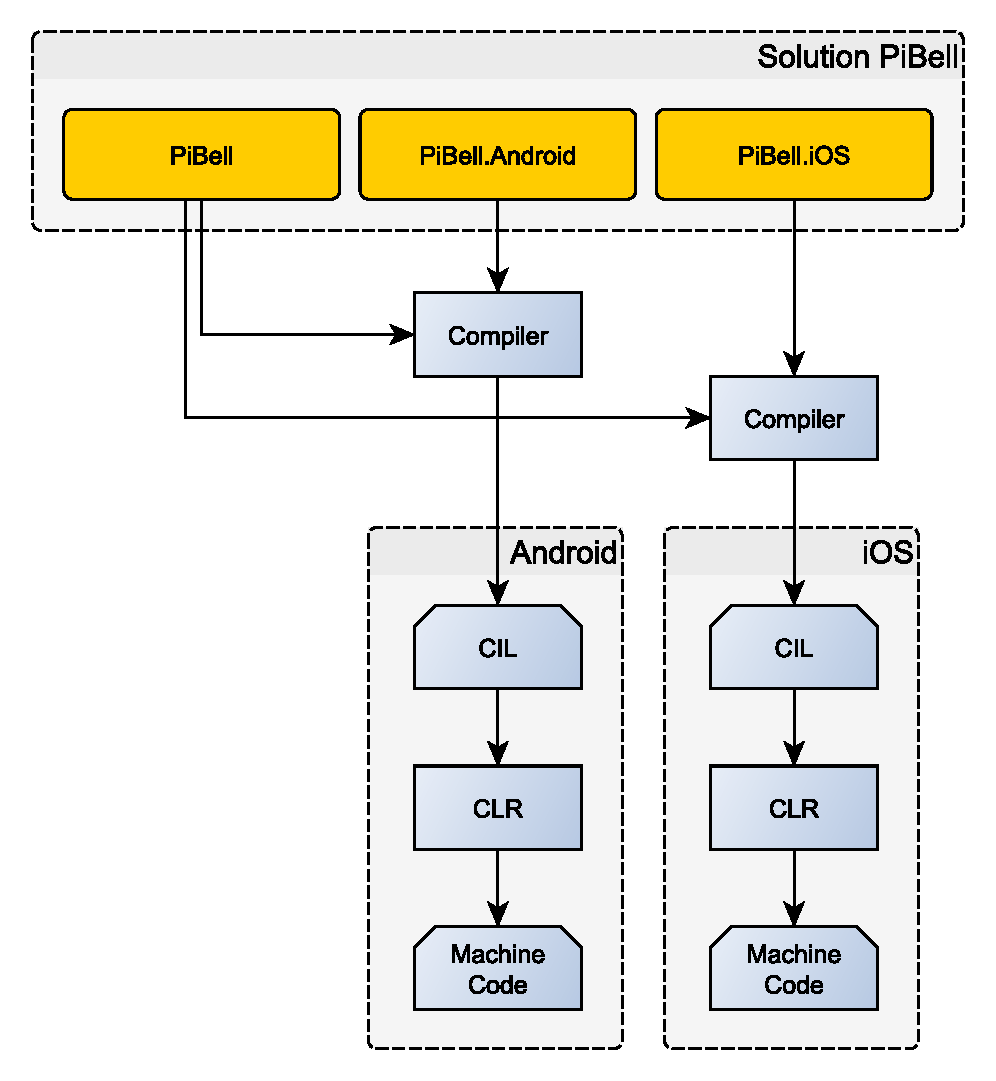
\includegraphics[width=0.9\linewidth]{images/auswahl_rahmenwerk/build-vorgang.pdf}
    \caption{Build-Vorgang einer Xamarin.Forms-Solution}
    \label{fig:build-forms}
\end{figure}

%Weg vom Programm zur binary
%microsoft VS2019
%frei zugänglich
%nur auf windows, kein linux-support
%...
\chapter{Verwendete Software-Module}
\section{Real Time Streaming Protocol}
\ac{rtsp} ist ein Netzwerkprotokoll zum Aufbauen und Verwalten von Netzwerkverbindungen zur Übertragung kontinuierlicher Medien-Daten (Streams).
Dieses Netzwerkprotokoll ist im \ac{ietf}-Dokument \citetitle{ietf-rtsp} festgelegt. 
Es wurde gemeinsam von \citeauthor{ietf-rtsp} entwickelt. \cite[vgl.][]{ietf-rtsp}\par

\subsection{RTSP Version 2}
Im Zuge dieser Diplomarbeit wird die erste Version des \ac{rtsp}-Protokolls verwendet.
Neben der verwendeten Version 1 existiert auch eine neue Version 2, welche im \ac{ietf}-Dokument \citetitle{ietf-rtsp-2} definiert ist. Die neue Version wurde von \citeauthor{ietf-rtsp-2} erarbeitet. \cite[vgl.][]{ietf-rtsp-2}\par
Es wurde dennoch die erste Version verwendet, da die Stationen dieses bereits verwenden und die neue Version nicht rückwärtskompatibel ist.\par

\ac{rtsp} wird in der Industrie vielseitig verwendet, um Live-Übertragungen von Überwachungskameras zu verwalten. Eine weitere Anwendung des \ac{rtsp} Protokolls ist das Streamen von Medien-Daten zu einem Server, der diese dann beispielsweise transcodiert oder aufnimmt.

\subsection{Anfragen-Aufbau}
Das \ac{rtsp}-Protokoll definiert mehrere Anfragen zur Verwaltung der Netzwerkverbindung.
Diese Anfragen werden, ähnlich wie beim \ac{http}, in unverschlüsseltem Plain-Text verschickt.
In Tabelle \ref{tab:rtsp-req} sind sämtliche Anfragen des \ac{rtsp}-Protokolls und deren Übertragungsrichtung aufgelistet.

\begin{table}
    \centering\begin{tabular}{r|c|c|l}
        \toprule
        \textbf{Methode}&\textbf{Richtung}         &\textbf{Objekt} &\textbf{Verbindlichkeit}\\
        \midrule
        DESCRIBE        &C$\rightarrow$S                    &P,S    &empfohlen\\
        ANNOUNCE        &C$\rightarrow$S, S$\rightarrow$C   &P,S    &optional\\
        GET\_PARAMETER  &C$\rightarrow$S, S$\rightarrow$C   &P,S    &optional\\
        OPTIONS         &C$\rightarrow$S, S$\rightarrow$C   &P,S    &erfordert, (S$\rightarrow$C: optional)\\
        PAUSE           &C$\rightarrow$S                    &P,S    &empfohlen\\
        PLAY            &C$\rightarrow$S                    &P,S    &erfordert\\
        RECORD          &C$\rightarrow$S                    &P,S    &optional\\
        REDIRECT        &S$\rightarrow$C                    &P,S    &optional\\
        SETUP           &C$\rightarrow$S                    &S      &erfordert\\
        SET\_PARAMETER  &C$\rightarrow$S, S$\rightarrow$C   &P,S    &optional\\
        TEARDOWN        &C$\rightarrow$S                    &P,S    &erfordert\\
        \bottomrule
    \end{tabular}\bigskip\par
    Richtung: C\dots Client, S\dots Server\par
    Objekt: P\dots Präsentation, S\dots Streams
    \caption[Anfrage-Arten des \ac{rtsp}-Protokolls \cite{ietf-rtsp}]
            {Anfrage-Arten des \ac{rtsp}-Protokolls \cite[aus dem Englischen übersetzt]{ietf-rtsp}}
    \label{tab:rtsp-req}
\end{table}
Das Aussehen einer solchen Anfrage wird anhand des Beispiels der DESCRIBE-Methode veranschaulicht.
Der Client beginnt die Anfrage mit dem \ac{url} des Medien-Streams, den er abrufen möchte und teilt dem Server mit, welche Formate er versteht.
\begin{minted}{text}
C->S: DESCRIBE rtsp://server.example.com/fizzle/foo RTSP/1.0
    CSeq: 312
    Accept: application/sdp, application/rtsl, application/mheg
\end{minted}
Der Server antwortet auf diese Anfrage mit dem Session Descriptor, der alle wichtigen Informationen des Medien-Streams beinhaltet, wie zum Beispiel Video- und Audio-Format, Übertragungsmethode, sowie allgemeine Informationen wie Titel und Beschreibung.
\begin{minted}{text}
S->C: RTSP/1.0 200 OK
    CSeq: 312
    Date: 23 Jan 1997 15:35:06 GMT
    Content-Type: application/sdp
    Content-Length: 376

    v=0
    o=mhandley 2890844526 2890842807 IN IP4 126.16.64.4
    s=SDP Seminar
    i=A Seminar on the session description protocol
    u=http://www.cs.ucl.ac.uk/staff/M.Handley/sdp.03.ps
    e=mjh@isi.edu (Mark Handley)
    c=IN IP4 224.2.17.12/127
    t=2873397496 2873404696
    a=recvonly
    m=audio 3456 RTP/AVP 0
    m=video 2232 RTP/AVP 31
    m=whiteboard 32416 UDP WB
    a=orient:portrait
\end{minted}

\section{LibVLC Sharp}
LibVLC ist ein Multimedia-Rahmenwerk der Non-Profit-Organisation VideoLAN, welche durch den VLC Media Player und dessen Funktionsumfang bekannt wurde. Der VLC Media Player funktioniert sozusagen als grafische Oberfläche zur LibVLC-Programmbibliothek.
Die Bibliothek beinhaltet viele nützliche Funktionen, darunter die folgenden:
\begin{itemize}
    \item Videos nahezu beliebigen Formates decodieren und darstellen
    \item Video und Audio aufnehmen und transcodieren für die weitere Verwendung
    \item Live-Streaming von Video-Daten, Webcam-Bild und Mikrofon-Ton.
\end{itemize}    
LibVLC ist eine Bibliothek für die C-Sprache. Um diese in einem C\#-Projekt verwenden zu können sind Bindings notwendig, welche Zugriff auf die C-Bibliothek geben.
LibVLC wurde von der Non-Profit-Organisation VideoLAN entwickelt und erstmals am 1. Februar 2001 veröffentlicht. \cite[vgl.][]{libvlc-release}\par

Im Xamarin.Forms-Projekt wird die zum Zeitpunkt der App-Entwicklung aktuelle Version 3.4.2 der LibVLC Sharp Bindings verwendet. Bindings erlauben es dem Programmierer, auf Programmbibliotheken zuzugreifen, welche für eine andere Sprache geschrieben wurden. Man kann sich Bindings wie Kleber vorstellen, der die Funktionen der einen Programmiersprache mit denen der anderen Sprache verbindet. Die Version 3.4.2 ist inzwischen nicht mehr die neueste Version, jedoch ist sie in Hinsicht auf Funktionalität deckungsgleich mit der neuesten Version.\par

\subsection{Erwähnenswerte Funktionen}
Die LibVLC-Sharp-Bindings ermöglichen die Verwendung des \ac{mvvm}-Modells, welches vom \ac{wpf}- und Silver\-light-Architekten John Gossman im Jahr 2005 auf seinem Blog vorgestellt wurde. \cite[vlg.][The Evolution of Model-View-ViewModel]{msdoc-mvvm}\par

Die Philosophie hinter diesem Modell ist, die Oberfläche (View) bis auf wenige Schnittstellen komplett vom eigentlichen Code zu trennen.
Dies ermöglicht es ohne größeren Aufwand, die Oberfläche zu ändern oder gar auszutauschen.
Folgende Terminologie wird in diesem Zusammenhang verwendet:
\begin{itemize}
\item Model … beinhaltet die Programmdaten. Meist werden einfache Klassen oder Strukturen hierfür verwendet.
\item View … Die grafische Oberfläche und deren Elemente wie Buttons, TextBoxen, und ähnliche
\item ViewModel … wandelt die Daten der Models so um, dass sie von der Oberfläche dargestellt werden können. ViewModel sind meist als Klasse ausgeführt.
\end{itemize}

Die Daten der Oberfläche und die Daten des Models bleiben zueinander konsistent.
Sobald sich ein Wert auf einer Seite ändert, wird er sofort auf der anderen aktualisiert.
Die hier beschriebenen Vorgänge sind in Abbildung \ref{fig:mvvm-flow} nochmals dargestellt.
\begin{figure}
    \centering
    \includegraphics[width=.9\linewidth]{images/software_module/MVVM.png}
    \caption{Datenfluss \ac{mvvm} \cite{ms-mvvm-flow}}
    \label{fig:mvvm-flow}
\end{figure}

Das \ac{mvvm}-Modell bietet sich auch an, wenn die Daten des Programms oft in eine andere Form gebracht werden müssen, bevor sie dargestellt werden können. Zum Beispiel wird vom Model die aktuelle Zeit als Ganzzahl abgespeichert, welche nur die vergangenen Millisekunden seit einem bestimmten Zeitpunkt zählt; um die Zeit allerdings darstellen zu können, muss diese Ganzzahl zuerst in ein lesbares Datumsformat gebracht werden. Diese Aufgabe würde das ViewModel übernehmen.

\subsection{Nachteile}
Sowohl die ursprüngliche LibVLC-Bibliothek, als auch die entsprechenden C\#-Bindings sind auf der offiziellen Dokumentationsseite nur spärlich dokumentiert. \cite[vgl.][]{libvlc-sharp-doc}\par

Beispielsweise verwenden alle Beispielprojekte der LibVLC Sharp Bindings das \ac{mvvm}-Modell, daher ist nicht bekannt, ob eine Implementierung ohne dieses Modell überhaupt möglich ist.
Weiters sind die einzelnen Funktionen zwar auf der Dokumentationsseite aufgelistet, allerdings nicht sehr ausführlich beschrieben. \cite[vgl.][]{libvlc-sharp-doc}

\subsection{Alternativen}
Während der Recherche wurden wenige Alternativen gefunden. Diese Alternativen sind jedoch seit langem nicht mehr in Entwicklung und sind daher nicht für die Verwendung empfohlen. Die LibVLC-Bibliothek ist momentan die einzige kostenfreie Variante, \ac{rtsp}-Streams mit Xamarin auf dem Mobilgerät abspielen zu können. Es gibt Bibliotheken von VASTreaming, jedoch sind diese kostenpflichtig zu erwerben, was für diese Diplomarbeit keine Option ist. \cite[vgl.][Pricing]{vastreaming}

\section{GStreamer}
\subsection{Modularität}
GStreamer ist ein extrem leistungsfähiges und vielseitiges Framework zur Erstellung von Medien-Streaming-Anwendungen.
Viele der Vorzüge des GStreamer-Frameworks liegen in seiner Modularität:
GStreamer kann neue Plugin-Module nahtlos integrieren.
Aber da Modularität und Leistungsfähigkeit oft mit einem Preis für eine größere Komplexität einhergehen, ist das Schreiben neuer Anwendungen nicht immer einfach.
\cite[aus dem Englischen übersetzt]{gstreamer}\par

GStreamer ist Pipeline-basiert, d.h. die Funktion wird mit einer Vielzahl von hintereinander geschalteten Filtern bestimmt.
Eine Pipeline hat immer einen Eingang (Source) und einen oder mehrere Ausgänge.
Zwischen diesen können sich beliebig viele Filter befinden, die unterschiedlichste Funktionen haben können:
\begin{itemize}
    \item Signale de- und encodieren (Codec, z.B. x264enc)
    \item Größe und Position von Videos verändern (Caps, z.B. video/x-raw)
    \item die Pipeline in zwei Teile auftrennen, z.B. in Video und Audio (Demux)
    \item Daten zu einem Netzwerk-Paket zusammenbündeln (z.B. rtph264pay)
    \item etc.
\end{itemize}
Ein Filter hat bestimmte Ein- und Ausgangsformate, die er unterstützt.
Als Beispiel nehmen wir den H264-Encoder:
dieser unterstützt für das Eingangssignal Raw-Video, also decodierte Binärdaten. Am Ausgang kommt logischerweise ein H264-codierter Video-Stream heraus.\par

\subsection{Version}
Das GStreamer-Rahmenwerk wird aktuell vom GStreamer-Team fortlaufend upgedatet und verbessert.
Die erste Version des GStreamer-Rahmenwerks wurde im Jahr 2001 mit der Versionsnummer 0.1.0 veröffentlicht.
Im Jahr 2012 kam eine große Umstellung, bei der grundlegende Teile des Rahmenwerks ausgetauscht wurden, wodurch einige Teile nicht mehr kompatibel waren.
Ab diesem Zeitpunkt begann die Versionsnummer mit 1.x.x, um die neuen Versionen deutlich von den Vorgängern abzutrennen.
Die aktuelle Version des GStreamer-Rahmenwerks zum Verfassungszeitpunkt dieser Arbeit ist die Version 1.16.2.\par

Aktuell wird die Version 1.16.2 verwendet. Da aber alle 1.x.x-Versionen mehr oder weniger miteinander kompatibel sind, kann sich das ändern, sobald ein neues Update veröffentlicht wird. Es gibt keinen besonderen Grund auf genau dieser Version zu bleiben.\par

\subsection{Alternativen}
Es wurden während der Recherche einige mögliche Alternativen für das GStreamer-Rahenwerk gefunden:
\begin{itemize}
    \item FFmpeg, ein Multimedia-Rahmenwerk, das vor allem im Bereich Transcodierung Verwendung findet. Es bietet alle Funktionen des GStreamer-Rahmenwerks an.
    \item LibVLC, die Grundlage des VLC Media Players, welche vor allem zur Wiedergabe verwendet wird. Diese Bibliothek kann zur Transcodierung und Live-Übertragung genutzt werden, ist allerdings nicht dafür optimiert.
\end{itemize}

\subsection{Vorteile}
GStreamer wird in diesem Projekt verwendet, da bei Live-Video-Übertragung möglichst wenig Latenz vorkommen soll.
Das GStreamer-Rahmenwerk ist in dieser Hinsicht den anderen Multimedia-Rahmenwerken weit voraus.
Zusätzlich gibt es von GStreamer keine einschränkenden Vorgaben, was Ein- und Ausgangsformat betrifft.
Es kann jede beliebige Quelle mit jedem beliebigen Output verknüpft werden, solange die richtige Pipeline verwendet wird.
Weiters ist das Projekt quelloffen, d.h. man ist in Bezug auf die Installationsdateien nicht auf den Hersteller angewiesen, sondern kann das Programm selbst für die jeweilige Plattform kompilieren, wenn der Hersteller das noch nicht getan hat.
Außerdem kann jeder Entwickler Vorschläge für Änderungen am Code sowie Bugfixes vorbringen.
\subsection{Funktionsweise}
Die detaillierte Funktionsweise des GStreamer-Rahmenwerks lässt sich am besten anhand eines realistischen Beispiels erklären.
In diesem Beispiel wird ein in Echtzeit generiertes Testvideosignal zuerst auf 1280x720 Pixel vergrößert und danach als H264-encodierter Stream via \ac{rtp} verschickt.
Mit dem Kommandozeilen-Programm \texttt{gst-launch-1.0.exe} kann ohne großen Aufwand eine Pipeline aufgebaut werden:
\begin{minted}{text}
    gst-launch-1.0 videotestsrc ! video/x-raw,width=1260,height=720,framerate=20/1 ! autovideoconvert ! queue ! x264enc tune=zerolatency bitrate=4096 speed-preset=superfast ! queue ! rtph264pay config-interval=1 mtu=1300 ! udpsink host=127.0.0.1 port=5000
\end{minted}
Der Filter \enquote{queue} wird hier verwendet, um vor und nach dem Encoding-Vorgang ein kurzes Video-Segment in einem Zwischenspeicher zu behalten. Dies ist notwendig, da der H264-Codec mehrere Video-Frames auf einmal komprimiert.

\subsection{Zusatzmodul}
gst-rtsp-server ist ein Zusatzmodul für das GStreamer- Rahmenwerk, welches die Verwendung des \ac{rtsp}-Protokolls für Server-Applikationen bereitstellt.
Mit diesem Modul können Medien-Streams, welche mit GStreamer verarbeitet wurden, mittels dem \ac{rtsp}-Protokoll dem Netzwerk bereitgestellt werden.

Das GitHub-Repository des Zusatzmoduls beinhaltet einige Beispielapplikationen, darunter auch \texttt{test-launch}.
Dieses Anwendungsbeispiel nimmt ähnlich wie das vorhin beschriebene \texttt{gst-launch-1.0} als Kommandozeilenargument eine GStreamer-Pipeline an.
Der resultierende Medienstream wird von der Anwendung in einen \ac{rtsp}-Stream verpackt und dem Netzwerk bereitgestellt.

\section{Live555 Proxy}
Ein \ac{rtsp}-Stream ist grundsätzlich eine Unicast-Verbindung zwischen Server und Client.
Falls mehrere Clients den gleichen Medien-Stream abrufen möchten, muss der Server diesen für jeden Client einzeln transcodieren und verschicken.
Dies stellt eine große Belastung für den Server und dessen Internetanbindung dar.
Mit Hilfe eines Proxy-Servers muss der Medien-Stream nur einmal verarbeitet werden, bevor er dann an die einzelnen Clients verteilt wird.\par

Der Live555 Proxy Server ist eine quelloffene Applikation, welche für genau diese Aufgabe von Live Networks Inc. entwickelt wurde.
Mit Hilfe des Live555 Proxy Servers wird ein \ac{rtsp}-Stream einmalig eingelesen und an alle verbundenen Clients verteilt.
Dadurch bleibt die \ac{cpu}-Belastung des Servers unabhängig von der Anzahl der verbundenen Clients, wodurch er unter Umständen mehrere verschiedene Streams bereitstellen könnte. Für jeden Medien-Stream, den der Server anbietet, wird eine weitere Live555-Proxy-Server-Instanz benötigt.\par

Das ursprüngliche Veröffentlichungsdatum des Live555 Proxy Servers konnte nicht gefunden werden.
Bei Analyse der Google-Such-Trends zum Begriff Live555 wurde festgestellt, dass Suchanfragen mit Oktober 2005 gestartet haben.
Daher lässt sich vermuten, dass das Programm kurz vor diesem Zeitpunkt veröffentlicht wurde. \cite[vgl.][Interest over time]{live555-trends}

Neben dem Live555 Proxy Server entwickelt das Unternehmen mehrere Projekte:
\begin{itemize}
    \item Live555 Media Server, mit dem lokale Medien-Dateien per \ac{rtsp} dem Netzwerk bereitgestellt werden können.
    \item liveCaster, zur Multicast-Übertragung von MP3-Dateien
    \item diverse Kommandozeilenprogramme zum Senden und Empfangen von Echtzeit-Streams
\end{itemize}
Die von Live Networks Inc. entwickelten Programme und Bibliotheken finden in vielen bekannten Applikationen Anwendung, darunter auch der VLC Media Player mit der dazugehörigen LibVLC. In diesem Programm werden die Live555-Bibliotheken zum Empfangen und Entschlüsseln von \ac{rtsp}-Streams genutzt.
\chapter{Push-Benachrichtigung}
\label{ch:push}
\section{Push Notification Service}
Eine Notification dient dazu den Benutzer über etwas zu informieren. Dies kann ein Kalender-Eintrag, eine eingetroffene SMS oder ein anderes Ereignis sein. Diese Art der Benachrichtigung wird meist über eine Local Notification erzeugt. Eine Local Notification wird aufgrund eines lokal am Gerät auftretenden Ereignisses ausgelöst. %bild
\begin{figure}[H]
    \centering\includegraphics[width=.5\linewidth]{images/xamarin/LocalNotification.png}
    \caption{Lokale Benachrichtigung}
\end{figure}

Im Gegensatz dazu dient eine Push Notification dazu, den Benutzer über ein externes Ereignis auf einem anderen Gerät aufmerksam zu machen. Diese Art der Benachrichtigung findet meist anwendung in der Katastrophenwarnung, um den Benutzer vor einer herannahenden Gefahr zu warnen.
Um den Benutzer also darüber zu informieren, dass jemand an der Haustür klingelt, wird eine Push Benachrichtigung verwendet, da das Anläuten-Ereignis bei der Außenstation erfolgt.
\begin{figure}[H]
    \centering\includegraphics[width=.5\linewidth]{images/xamarin/PushNotification.png}
    \caption{Push-Benachrichtigung}
\end{figure}

\subsection{Funktionsweise}
Eine Push Notification wird immer von einem sogenannten Push Notification Service an ale Zielgeräte geschickt.
Dieser Service wird vom jeweiligen Betriebssystem-Hersteller bereitgestell.
Im Fall der hier entwickelten App sind das Google und Apple, mit ihren Push Notification Services GCM und APNs.\par

Der Service ist dafür verantwortlich die Benachrichtigung an alle registrierten Zielgeräte zu schicken.
Wenn das Zustellen nicht möglich ist, bricht der Service die Zustellung nach mehreren Versuchen für dieses Gerät ab.
Alle anderen Geräte erhalten die Benachrichtigung.
Daher ist es nicht es nicht sichergestellt, dass eine Push-Benachrichtigung bei jedem Gerät ankommt.\par

Zusätzlich zum Nachrichtentext können bei einer Push Notification zusätzliche Daten mitgeschickt werden. Diese können zum Beispiel die App über die genaue Benachrichtigungsursache informieren.

\section{AppCenter Push}
AppCenter Push hat in erster Linie die Funktion, den Zugriff auf die verschiedenen Push Notification Services zu vereinheitlichen und damit einfacher zu gestalten.
Microsoft AppCenter verwaltet alle Server-API-Schlüssel, Zielgerätelisten und ähnliche Einstellungen, um den Prozess des Benachrichtigung-Sendens zu vereinfachen.
AppCenter Push ist entweder über das Web-Interface unter \url{https://appcenter.ms/} oder über die AppCenter API erreichbar und verwendbar.\par

Die AppCenter Push SDK abstrahiert den ganzen Prozess der Geräte-Registration, des Registrieren des Eingangs-Events und versteckt alles hinter einer einzelnen simplen Funktion \texttt{AppCenter.Start(„{App Secret}“, typeof(Push));}. Das App Secret ist der von AppCenter zugewiesene Schlüssel mit dem sichergestellt wird, dass das Gerät für das richtige AppCenter Projekt registriert wird.
Ohne diese SDK müsste in der App viel mehr konfiguriert werden, was einen höheren Programmieraufwand und größere Fehlerrate darstellt. Außerdem würde das Rad neu erfunden werden.\par

In der entwickelten App wird die Appcenter-SDK-Version 2.6.4 verwendet. Zu beachten ist, dass Appcenter Push nicht mehr weiterentwickelt wird und irgendwann dieses Jahr der Service abgeschaltet wird, wie es John Wargo in seinem Blog-Post am 3. Februar 2020 schrieb. Als Alternative wird von Microsoft der Azure Notification Hubs dienst angeboten. Bevor Appcenter Push endgültig terminiert wird, will Microsoft detaillierte Anleitungen zum Umstieg auf Azure bereitstellen.\par

\subsection{Konfiguration des SDK}
Um Appcenter Push in der Applikation verwenden zu können müssen mehrere NuGet-Pakete installiert werden.
Das AppCenter Paket beinhaltet alle Kernfunktionen wie AppCenter.Start(), das AppCenter-Push-Paket erweitert das Grundpaket um Push-bezogene Funktionen und Datentypen.
\begin{table}[H]
    \centering\begin{tabular}{|c|c|c|c|}
        \hline
        NuGet-Paket & PiBell & PiBell.Android & PiBell.iOS\\
        \hline
        AppCenter & Ja & Ja & Ja\\
        AppCenter Push & Ja & Ja & Ja\\
        \hline    
    \end{tabular}
    \caption{Installation NuGet-Pakete}
\end{table}
\chapter{Programm-Dokumentation}
% Im Juni 2000 stellte das Unternehmen Microsoft das \ac{dotnet} vor.
% Kurz darauf wurde von Miguel de Icaza das sogenannte Mono-Projekt als Open-Source gestartet, welches eine Linux-Version des \ac{dotnet} darstellen soll.
% Am 16. Mai 2011 kündigt Miguel de Icaza an, dass das Mono-Projekt vom Unternehmen Xamarin weiterentwickelt wird, wobei einige wichtige Mitglieder des Mono-Entwickler-Teams weiterhin daran beteiligt sind.

% Das Unternehmen Xamarin wurde mit der Absicht gegründet, Software auf mobile Geräte zu vertreiben. 
\label{ch:prog-doc}
\section{Übersicht}
Das im Zuge dieser Diplomarbeit entwickelte Software-Projekt basiert auf einer der von Microsoft bereitgestellten Xamarin.Forms-Vorlagen, welche als Teil von Visual Studio bereitgestellt werden.
Es gibt mehrere Auswahlmöglichkeiten, wobei alle Vorlagen bis auf \enquote{Blank} Beispielcode beinhalten.
Da der Beispielcode der anderen Vorlagen für dieses Projekt nicht relevant ist und ohnehin gelöscht werden müsste, wird die \enquote{Blank}-Vorlage verwendet.
Diese Vorlage beinhält nur eine Haupt-Oberflächenseite ohne jeglichen Beispielcode.

Der immer wieder vorkommende Name PiBell ist eine freigeistliche Erfindung. PiBell ist der Projektname, der sich aus \acl{rpi} und \enquote{Bell}, dem englischen Wort für Klingel oder Glocke, zusammensetzt.

Visual Studio organisiert alle Programmteile in einer sogenannten Solution, welche den Projektnamen trägt. In diesem Fall beinhält die Solution \enquote{PiBell} drei Programmteile oder \enquote{Projects}:
\paragraph{PiBell} ist das portable Projekt, auch .NET-Standard-Projekt genannt.
Dieses beinhaltet den ganzen plattformunabhängigen Code, sowie die Definition der UI-Oberfläche mittels XAML-Dateien.
In diesem Projekt befindet sich der größte entwickelte Code-Anteil, da die meisten Funktionen, wie das Abspielen von Videos mit Hilfe der LibVLC-Bindings, plattformunabhängig funktionieren und deswegen geteilt werden können.

\paragraph{PiBell.Android} beinhaltet allen Code, der plattformspezifisch für Android geschrieben wurde.
Unter anderem ist hier enthalten die Android-Implementation des Mikrofon-Auf\-nahme-Services, sowie das Berechtigungs-Management.
Die Mikrofon-Aufnahme erfolgt auf einer sehr hardwarenahen Ebene, was die plattformabhängigkeit erklärt.

\paragraph{PiBell.iOS} beinhaltet wie PiBell.Android den plattformspezifischen Code für die iOS-Platt\-form. Aufgrund mangelnder Entwicklungswerkzeuge wurde dieser Teil nicht großartig behandelt.\par

\begin{figure}[H]
\centering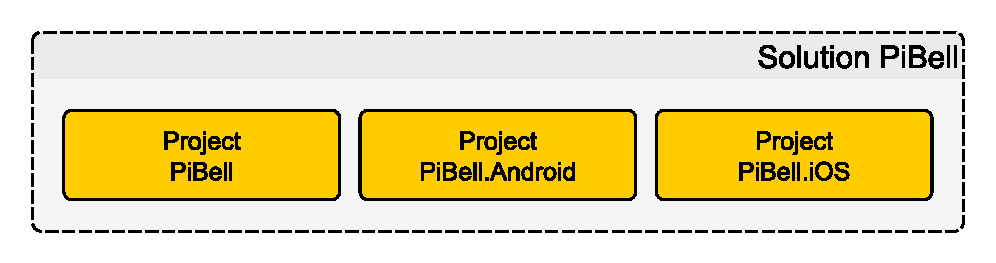
\includegraphics[width=0.9\linewidth]{images/xamarin/struktur.pdf}
\caption{Aufbau der Solution}
\end{figure}

%besteht aus drei teilen
%- portable project/.net standard project
%   plattformunabhängiger teil, oberfläche, ...
%- Android project
    %android-spezifischer teil, berechtigungen, ...
%- iOS project
    %iOS-spezifischer Teil, ...
%project-name PiBell -> erfindung, leitet sich aus raspberry und Türglocke ab
%
\section{Portable Project}
\subsection{App.xaml.cs}
\begin{lstlisting}[firstnumber=17]
public App()
{
    InitializeComponent();
    Core.Initialize();
    MainPage = new MainPage();


    AppCenter.LogLevel = Microsoft.AppCenter.LogLevel.Verbose;
    AppCenter.Start("android=2234efba-9d8c-45ec-bfad-f78aaa6ba632;" +
                    "uwp={Your UWP App secret here};" +
                    "ios={Your iOS App secret here}",
        typeof(Analytics), typeof(Crashes), typeof(Push));
}
\end{lstlisting}
\paragraph{19/20:} Die Funktionen InitializeComponent() und Core.Initialize sind vorgefertigte Funktionen; diese sind zu verwenden um die Applikation und alle benötigten Bibliotheken zu initialisieren.
\paragraph{21:} Die Anweisung MainPage = new MainPage() erzeugt eine neue Oberfläche, mit der der Benutzer mit der App interagiert. Diese Oberfläche erscheint nach dem App-Start am Bildschirm und passt sich automatisch der physikalischen Bildschirmgröße an.
\paragraph{24-28:} Mit AppCenter.LogLevel kann festgelegt werden, welche Log-Nachrichten angezeigt werden. In diesem Fall werden Alle Nachrichten aktiviert.
Anschließend wird das AppCenter SDK mit AppCenter.Start(..) gestartet. Am Ende dieser Anweisung werden alle Module (Analytics, Crashes und Push), die dazu gestartet werden sollen angegeben.

\subsection{MainPage.xaml}
%vlcht. Zu Xamarin im Allgemeinen
In einer XAML-Datei wird das Aussehen der Oberfläche nach dem WYSIWYM-Prinzip beschrieben. Das Format ähnelt sehr einer XML-Datei, in der Hinsicht, dass ein Element mit einer spitzen Klammer (<) beginnt und mit einem Schrägstrich und einer spitzen Klammer (/>) endet. Einige Elemente, wie zum Beispiel Listen oder ein Grid, können sogenannte Kind-Elemente beinhalten.
\begin{lstlisting}[firstnumber=3,language=xml]
<ContentPage xmlns="http://xamarin.com/schemas/2014/forms"
             xmlns:x="http://schemas.microsoft.com/winfx/2009/xaml"
             xmlns:local="clr-namespace:PiBell"
             xmlns:piBell="clr-namespace:PiBell;assembly=PiBell"
             xmlns:shared="clr-namespace:LibVLCSharp.Forms.Shared;assembly=LibVLCSharp.Forms"
             x:Class="PiBell.MainPage"
             Title="Main Page"
             BackgroundColor="#ff1b1b1b">
\end{lstlisting}
\paragraph{3-8:} Am Anfang der XAML-Datei wird der allgemeine Seiten-Typ, gemeinsam mit einigen Quell-Abkürzungen (Namenspräfix für Xamarin-fremde Elemente) definiert. In diesem Fall handelt es sich um eine simple ContentPage mit den Standard-Abkürzungen. Zur Verwendung der LibVLC wurde in Zeile 7 eine zusätzliche Quelle definiert. Die neu hinzugefügte Quelle erlaubt den Zugriff auf Elemente wie die VideoView, welche ein Video als Teil der Oberfläche darstellt.
\paragraph{9:} Mit x:Class wird die Programmklasse angegeben, die den Code der Oberfläche beinhält. In dieser Klasse finden sich alle Event-Handler für jegliche Oberflächenereignisse, wie das drücken eines Buttons.
\paragraph{10:} Das festlegen der Title-Variable ist in diesem Fall optional. Falls eine Master-Detail-Page-Struktur verwendet werden würde, wäre der Titel oben in der Kopfzeile der App zu sehen. Da es sich hier aber um ein Sigle-Page-Layout handelt, ist der Titel nicht zwingend notwendig.
\paragraph{11:} Mit der Variable BackgroundColor wird die Hintergrundfarbe der Oberfläche definiert. Die gewünschte Farbe wird als HEX-Zahl mit dem Format Alpha-Rot-Grün-Blau angegeben. Der Alpha-Wert legt die Durchsichtigkeit der Farbe fest. Es wurde sich für ein dunkles Design entschieden, da dieses in einer wenig beleuchteten Umgebung die Augen besser schont.

\begin{lstlisting}[firstnumber=12,language=xml]
<ContentPage.Content>
    <Grid Margin="10" x:Name="MainGrid">
        <Grid.RowDefinitions>
            <RowDefinition Height=".7*" />
            <RowDefinition Height="3*" />
            <RowDefinition Height="2*" />
        </Grid.RowDefinitions>
        <Grid.ColumnDefinitions>
            <ColumnDefinition Width="*" />
        </Grid.ColumnDefinitions>
\end{lstlisting}
\paragraph{12:} Mit dieser Zeile wird das Element ContentPage.Content geöffnet. Content steht hier für den gesamten Oberflächeninhalt, also alle Schaltflächen und Anzeigen.
\paragraph{13-21:} Als erstes und einziges Kind-Element von ContentPage.Content wird die Komponente Grid gewählt. Diese ermöglicht es, mehrere Kind-Elemente in einer schachbrettartigen Anordnung zu organisieren. Hierfür werden mit Hilfe der Row- und ColumnDefinitions die Höhen und Breiten der einzelnen Zeilen und Spalten festgelegt. Der Stern (*) in der Längenangabe bedeutet relatives Maß bezogen auf die verfügbare Breite bzw. Höhe.
\begin{lstlisting}[firstnumber=23,language=xml]
<Entry x:Name="EditMrl" Text="{Binding Mrl, Mode=TwoWay}" Grid.Row="0" Grid.Column="0" TextColor="White" />

<shared:VideoView x:Name="VideoView" Grid.Column="0" Grid.Row="1" MediaPlayer="{Binding MediaPlayer}"/>
\end{lstlisting}
\paragraph{23:} Hier wird das erste eigenständige Oberflächen-Element erzeugt. Es handelt sich um ein Text-Eingabe-Feld (Entry), mit dem zu Testzwecken die Serveradresse eingegeben werden kann. Dies ist notwendig, da die finale Serveradresse noch nicht bekannt ist und sich diese im Zuge der Entwicklung ständig ändert. Für den späteren Betrieb könnte dieses Problem umgangen werde, indem die aktuelle Server-Adresse per Push-Benachrichtigung mitgeschickt wird. Hier ist auch eine Anwendung des MVVM-Modells erkennbar: es wird mit Hilfe des Binding-Schlüsselwortes der Speicherort des angezeigten Textes festgelegt. Mode=TwoWay beschreibt die Richtung der Synchronisierung der Daten. Egal, ob sich der Wert im Speicher oder der Wert in der Anzeige ändert, wird die jeweils andere Seite aktualisiert. Mit Grid.Row und Grid.Column wird die Position im vorhin definierten Grid gesetzt.
\paragraph{25:} Das zweite Oberflächen-Element, eine VideoView der LibVLC, wird hier erzeugt. Da die Komponente VideoView nicht standardmäßig in Xamarin enthalten ist, wird das am Anfang der Datei definierte Namenspräfix „shared:“ benötigt.

\begin{lstlisting}[firstnumber=36,language=xml]
<ImageButton x:Name="BtConnect" Source="call.png" BackgroundColor="LimeGreen" Grid.Row="0"
             Grid.Column="0" Margin="10"
             Clicked="BtConnect_Clicked"/>
\end{lstlisting}
\paragraph{36:} Ein ImageButton kann im Vergleich zu einem normalen Button als Inhalt ein Bild anzeigen. Die Bildquelle wird mit der „Source“-Property gesetzt. Es gibt mehrere mögliche Bildformate, wobei hier PNG aufgrund von Transparenz-Unterstützung gewählt wurde. Ohne Definition der „BackgroundColor“ würde der ImageButton mit der Default-Farbe grau gefüllt werden.
\paragraph{38:} Mit dem EventHandler „Clicked“ kann die Funktion, die aufgerufen wird wenn der ImageButton gedrückt wird, spezifiziert werden.
\begin{lstlisting}[firstnumber=43,language=xml]
<ImageButton x:Name="BtToggleSpeaker" Source="SpeakerMute.png" BackgroundColor="Transparent"
             Grid.Row="1" Grid.Column="0" Margin="10"
             Clicked="BtToggleSpeaker_Clicked">
    <VisualStateManager.VisualStateGroups>
        <VisualStateGroup x:Name="SpeakerStates">
            <VisualState Name="Mute">
                <VisualState.Setters>
                    <Setter Property="Source"
                            Value="SpeakerMute.png" />
                </VisualState.Setters>
            </VisualState>
            <VisualState Name="Unmute">
                <VisualState.Setters>
                    <Setter Property="Source"
                            Value="SpeakerUnmute.png" />
                </VisualState.Setters>
            </VisualState>
        </VisualStateGroup>
    </VisualStateManager.VisualStateGroups>
</ImageButton>
\end{lstlisting}
\paragraph{47-62:} Mit dem VisualStateManager können für die meisten Oberflächen-Elemente bestimmte Zustände definiert werden (z.B. wenn sie gedrückt sind). Hier werden zwei Zustände definiert, die das angezeigte Bild dem Lautsprecher-Zustand anpassen.
\begin{figure}[H]
    %grafik eventuell oben abschneiden
    \centering\includegraphics[width=.9\linewidth]{images/xamarin/VisualStateManager.png}
    \caption{VisualStateManager}
\end{figure}
Die hier beschriebenen Konzepte werden mehrmals verwendet, um die Oberfläche aufzubauen. Die Datei als Gesamtheit ergibt die in Bild xx gezeigte Oberfläche:
\begin{figure}[H]
    %grafik eventuell oben abschneiden
    \centering\includegraphics[width=.9\linewidth]{images/xamarin/MainPage.png}
    \caption{App-Oberfläche}
\end{figure}

%main.xaml.cs
\section{PiBell.Android}
%audio recording service
%permissions
%OnPause(), OnRestart()
\section{PiBell.iOS}
\chapter{Software-Ausblick}
\section{Gesicherte Verbindung}% VPN-Zugriff
Die im Zuge dieser Arbeit entwickelte Applikation verschickt bzw. empfängt alle Daten-Streams unverschlüsselt und ohne Benutzerverifizierung.
Bevor die Applikation im Feld verwendet werden kann, sollte eine gesicherte Verbindung zum Server konfiguriert werden.
Dies kann zum Beispiel per \ac{vpn} erfolgen.
Hier wird ein verschlüsselter Tunnel zu einem gemeinsamen Server aufgebaut, in dem alle Daten verschickt werden.
Dieses neu erzeugte Netzwerk ist virtuell, d.h. es existiert nur in der Softwarewelt und benötigt keine zusätzliche physikalische Verbindung.\par
Man könnte entweder auf kommerzielle \ac{vpn}-Anbieter zurückgreifen oder mit Open\-VPN und einem eigenen Server eine gesicherte Verbindung ermöglichen.
Im letzteren Fall kann auch der Medienserver die Rolle des \ac{vpn}-Servers übernehmen.
\section{Weitere mobile Plattformen}
Neben dem ausprogrammierten Android-System gibt es noch das weit verbreitete iOS der Apple-Geräte.
Mit Xamarin.Forms lässt sich dieses verglichen mit anderen Entwicklungsmethoden einfach unterstützen.
Es muss lediglich der plattformspezifische Teil auf die neue Plattform portiert werden, während das portable Projekt unverändert bleibt.
Dies bedeutet, dass analog zum PiBell.Android ein Projekt PiBell.iOS geschrieben werden muss, um die Plattform zu unterstützen.
In diesem Projekt müssen alle Funktionen des Android-Teils repliziert werden.
Wichtig für die Entwicklung ist auch, dass die Endgeräte zum Übertragen und Testen verfügbar sind.
Im Fall der iOS-Plattform wird ein Apple Mac für die Übertragung und ein Apple iPhone zum Testen benötigt.\par

Für Testzwecke kann die Applikation auf bis zu fünf iPhones installiert und getestet werden.
Wenn die App schlussendlich veröffentlicht werden soll, ist eine kostenpflichtige Mitgliedschaft beim Apple Developer Program notwendig.
Diese beläuft sich auf etwa USD 99 pro Jahr \cite[vgl.][Integrated Development Environment Availability]{msdoc-xamarin-fundamentals}
%\blindtext
\cleartoverso

\renewcommand{\authorName}{\MatthiasMair}
\part{Hardware - \MatthiasMair}
\chapter{Ausgangssituation}
\section{Hardware-Konfiguration}
Die aktuelle Hardware der Station setzt sich aus mehreren Einzel-Platinen mit unterschiedlichen Betriebsspannungen zusammen:
\begin{itemize}
    \item Mikrofon-Vorverstärker-Platine, die das Signal des Kondensator-Mikrofons verstärkt, bevor es zum \ac{rpi} weitergeleitet wird. Diese Platine wird mit einer Spannung von 5VDC betrieben.
    \item Lautsprecher-Verstärker-Platine, die für die Verstärkung der wiederzugebenden Audiosignale des \ac{rpi} zuständig ist. Die verstärkten Signale werden direkt an den Lautsprecher der Station übergeben. Diese Platine benötigt eine Versorgungsspannung von 24VDC.
\end{itemize}
Die elektrische Versorgung der Station erfolgt mittels \ac{poe} bei einer Speisespannung von etwa 30VDC.
Alle Platinen sind mit Heißkleber in der Station montiert.

\section{Problemdefinition}
\paragraph{Systemstabilität:} %poe
In der aktuellen Konfiguration kommt es immer wieder zu unvorhersehbaren und unkontrollierten Systemabstürzen.
Die betroffene Station reagiert weder auf eingehende Signale, noch erfolgt irgendeine Form der Informationsausgabe.
Dieser Zustand lässt sich nur durch ein Zurücksetzen des Prozessors beenden.
Die Abstürze sind bei der am weitesten von der Spannungsversorgung entfernten Station am häufigsten zu beobachten.
Dieser Fehler tritt in unregelmäßigen Abständen von bis zu mehreren Monaten auf.
Die betroffene Station weist keinen Hardware-Unterschied zu den anderen Stationen auf.
Daher lässt sich vermuten, dass die Länge und Art der Verkabelung mit diesem Phänomen in Zusammenhang steht.

\paragraph{Komplexer Aufbau:} %einzelplatinen
Die aktuelle Hardware-Konfiguration verwendet einige Einzelplatinen, die miteinander über eine fliegende Verdrahtung verbunden sind.
Dies reduziert die Übersichtlichkeit des Stationsinneren und birgt die Gefahr von fehlerhafter Verdrahtung in sich.
Durch die fliegende Verdrahtung ist kein einheitliches Erscheinungsbild des Stationsinneren gewährleistet.

\paragraph{Brumm-Schleife:} %gnd-loop
Die aktuelle Verdrahtung führt zu einer Masseschleife.
Diese erzeugt ein konstantes Störgeräusch.
Über die Verstärkerschaltung führt dies zu einem unerträglichen Brumm-Ton.
In der aktuellen Hardware-Konfiguration wird das Problem mit einer Massetrennung nach dem Ausgang des \ac{rpi} umgangen.
Dieser zusätzliche Baustein wurde fliegend verdrahtet und mit Heißkleber befestigt.

Folgend ein Bild der aktuellen Station und deren Verdrahtung.
\begin{figure}[H]
    \centering
    \includegraphics[width=.9\linewidth]{images/ist_situation/fliegender_aufbau.pdf}
    \caption{Unübersichtliche Verdrahtung}
\end{figure}
\chapter{Technische Grundlagen}
\wip
\section{Power over Ethernet}
Bei Power over Ethernet wird die Energieversorgung über eine herkömmliche Cat5-Ethernetleitung mitgeführt.
Dadurch wird eine weitere Versorgungsleitung eingespart.
Eine Ethernet Leitung besteht aus acht Adern, wobei je zwei Adern zu einem Adernpaar verdrillt sind.
Je nach Geschwindigkeit der Datenübertragung werden nur vier oder alle acht Adern für die Datenübertragung verwendet.
Das bedeutet, bei geringeren Übertragungsraten können die freien Adern zur Versorgung genutzt werden.
Wenn alle acht zur Datenübermittlung verwendet werden, müssen vier Adern für Datenübertragung \emph{und} Energieversorgung genutzt werden.\par

Grundsätzlich wird zwischen vier verschiedenen Typen unterschieden:
\paragraph{Type 1, \ac{poe}:}
Der Standard \ac{ieee} 802.3af gilt nur für 10 Mbit/s und 100 Mbit/s.
Das bedeutet, dass nur die Adernpaare 1/2 und 3/6 für die Datenübertragung genutzt werden und die beiden anderen Adernpaare unbenutzt sind.
Je Adernpaar ist ein Strom von maximal 175 mA vorgesehen. Bei zwei Adernpaaren ist das in Summe ein Strom von 350 mA.
Beim Einschalten sind kurzzeitig 400 mA erlaubt.
Die maximale Leistungsaufnahme beträgt 15,4 Watt pro Switch-Port.

\paragraph{Type 2, \ac{poep}:}
Mit \ac{ieee} 802.3at eignet sich Power-over-Ethernet auch für 1000 Mbit/s (Gigabit).
Gleichzeitig wird die Leistung fast verdoppelt.
\ac{ieee} 802.3at verspricht eine Leistung bis 25,5 Watt pro Port.
Dabei wird die Minimalspannung von 44 auf 50 Volt erhöht.
Der maximale Strom wurde von 350 mA auf 600 mA erhöht.
Bei diesen hohen Leistungen wird ein Cat5e/6-Kabel empfohlen.

\paragraph{Type 3 \& 4, \ac{poepp}:}
Den Standard \ac{ieee} 802.3bt bezeichnet man als Four-Pair-Power-over-Ethernet. Die Kurzschreibweise \ac{poepp} oder \aca{poepp}.
Bisher nutzt Power-over-Ethernet nur zwei der vier Aderpaare eines Twisted-Pair-Kabels. Mit \ac{poepp} werden alle Adern der vorhandenen Kabel zur Leistungsübertragung verwendet. Damit steigt die Leistung auf 70 bis 100 Watt.

Aus den verschiedenen Typen ergeben sich zwei Arten der Energiespeisung:
\paragraph{Spare-Pairs-Verfahren:}
Das Spare-Pairs-Verfahren verwendet die beiden unbenutzten Adernpaare im Kabel (4/5 und 7/8) für die Stromversorgung. Die Übertragung von Strom und Daten sind voneinander getrennt. Diese Art kann nur bei Type 1 und Type 2 verwendet werden.

\paragraph{Phantom-Speisung:}
Bei der Phantom-Speisung werden die datenführenden Adern im Kabel verwendet. Phantom-Speisung bedeutet, dass der Strom für die Energieversorgung dem Datensignal überlagert wird. Das Power-Device muss die Entkopplung übernehmen, was fehleranfällig, aufwendig und teuer ist.
Wenn alle Adernpaare des Kabels für die Datenübertragung verwendet werden, d.h. es wird Type 3 oder Type 4 angewendet, dann ist man zwangsläufig auf die Phantom-Speisung angewiesen. Hierbei ist der Strom pro Adernpaar und somit die Gesamtleistung begrenzt.

\begin{table}[H]
	\centering
	\begin{tabular}{lccc}
		\toprule
		Type & \ac{poe} & \ac{poep} & \ac{poepp} \\
		\midrule
		Ausgangsspannung & 36-57 V & 42.5-57 V & 42.5-57 V \\
		\midrule
		Ausgangsstrom Betrieb & 350 mA & 600 mA & 2x 960 mA \\
		\midrule
		Ausgangsstrom Startmodus & 400 mA & 400 mA & ? \\
		\midrule
		Leistung der (\ac{pse})-Versorgung & max. 15.4 W & max. 30 W & 45/60/75/90 W \\
		\midrule
		Leistung am Endgerät (\ac{pd}) & max. 12.95 W & max. 25.5 W & 40/51/62/71 W\\
		\midrule
		\ac{pse}-Klasse & 1, 2, 3 & 4 & 5, 6, 7, 8 \\
		\midrule
		unterstützte Endgeräte (\ac{pd}-Type) & 1 & 1 und 2 & 1, 2, 3, 4 \\
		\midrule
		Benutzte Adernpaare & 2 & 2 & 2 und 4 \\
		\bottomrule
	\end{tabular}
	\caption{Vergleich PoE-Typen \cite[vgl.][]{elektropraktiker-poe}}
	\label{tab:poe-types}
\end{table}

\section{Spannungsregler}
Ein Spannungsregler stabilisiert eine elektrische Spannung.
Er wird eingesetzt, wenn eine konstante Betriebsspannung benötigt wird.
Grundsätzlich arbeitet ein Spannungsregler mit einem Leistungstransistor, der so angesteuert wird, dass die gewünschte Ausgangsspannung zu Stande kommt.\par

Es gibt zwei Arten von Spannungsregler:
\paragraph{Linearregler:}
Beim Linearregler wird der Leistungstransistor als veränderbarer Widerstand genutzt.
Über einen Regelkreis wird eine Veränderung der Ausgangsspannung, z.B. Laständerung, festgestellt.
Daraufhin ändert der Transistor seinen Innenwiderstand, um die Veränderung auszugleichen.\par

\paragraph{Schaltregler:}
Der Schaltregler hingegen nutzt den Leistungstransistor als Schalter.
Er schaltet mit einer Frequenz von mehreren kHz bis MHz und erzeugt somit ein \ac{pwm} Signal.
Dieses Signal wird anschließend mit einer Induktivität geglättet, um einen konstanten Strom zu erzielen.\par

Bei der \ac{pwm} wird das Verhältnis zwischen der Einschaltzeit und Periodendauer eines Rechtecksignals bei fester Grundfrequenz variiert. Das Verhältnis zwischen der Einschaltzeit tein und der Periodendauer T=tein+taus wird als das Tastverhältnis p bezeichnet. (laut \ac{din}-\ac{iec} 60469-1: Tastgrad) (engl. Duty Cycle, meist abgekürzt DC, nicht zu verwechseln mit Direct Current = Gleichstrom). \cite[Einleitung]{mikrocontroller-spannungsregler}\par

\section{Surface Mounting Technology}
Bei der klassischen \ac{tht}-Technologie werden die Bauteilanschlüsse durch Löcher in der Platine gesteckt und mit kreisförmigen Lötpads auf der gegenüberliegenden Seite verlötet.
Im Gegensatz dazu sind bei \ac{smd}-Platinen Bauteile und Lötpads auf derselben Platinenseite, weshalb keine Bohrungen mehr erforderlich sind.
Die Bauteilanschlüsse werden flach mit dem rechteckigen Lötpad verbunden.
Die Verlötung findet mithilfe von Heißluft statt.
Die fertig bestückten Platinen werden in einen Reflow-Ofen gelegt und auf die Schmelztemperatur der Lötpaste erhitzt.

\subsection{Entwicklung}
In den 1960ern wurde die Oberflächenmontagetechnik (\ac{smt}) von \ac{ibm} entwickelt und fand ihre ersten Anwendungen in den Saturn- und Apollo-Missionen.
In den 1970ern wurde die \ac{smt} erstmals genormt, wodurch sich die Technologie im kommerziellen Sektor verbreiten konnte.
Die \ac{smt} bietet gegenüber der herkömmlichen \ac{tht} einige Vorteile:
\paragraph{Vorteile:}
\begin{itemize}
	\item Miniaturisierung, aufgrund der geringeren Größe der Bauteile können Platinen und somit auch Endgeräte kleiner und kompakter gebaut werden.
	\item Auch das Gewicht wird durch die Verkleinerung der Bauelemente stark reduziert.
	\item Der Bauteilabstand kann verkleinert werden, dadurch verbessert sich der Platzverbrauch weiter.
	\item Die Hochfrequenzeigenschaft wird durch die kürzeren Übertragungswege zwischen den Bauteilen verbessert.
	\item Die Fertigung der Platinen kann mit \ac{smd} besser automatisiert werden, da die Positionierung der Bauelement nicht so genau sein muss, wie bei \ac{tht}.
	Die Bauteile werden beim Verlöten durch die Oberflächenspannung des Lötzinns in die korrekte Position gezogen.
	\item Einfache doppelseitige Bestückung von Platinen, da kein Platz von Anschlüssen von Bauteilen auf der anderen Platinenseite verbraucht wird.
\end{itemize}

\paragraph{Nachteile:}
\begin{itemize}
	\item Anschlüsse an der Unterseite von Bauteilen können nur durch Röntgen überprüft werden.
	\item Das Heißluftlötverfahren erhitzt nicht nur die Lötstelle, sondern das gesamte Bauteil.
 	Dadurch besteht ein höheres Risiko, dass dieses beim Anlöten zerstört wird.
 	\item Große Bauelemente benötigen zusätzliche Fixierung, da die Lötstelle der mechanischen Belastung nicht standhält.
	Aufgrund der vielen Vorteile gegenüber \ac{tht} fand die \ac{smt} in der Digital- und Computertechnik anfänglich häufige Anwendung.
	Anfang der 1980er begannen die ersten Unternehmen mit der automatischen Fertigung von \ac{smd}-Platinen, wodurch die Herstellungskosten weiter gesenkt wurden.	
\end{itemize}

\subsection{Bauteilcodes}
Grundsätzlich werden alle elektronischen Bauteile in die beiden Untergruppen aktive und passive Bauelemente unterteilt.\par

Aktive Bauelemente können Signale verstärken oder erzeugen. Die benötigte Energie kommt aus einer zusätzlichen Versorgung durch elektrischer oder einer anderen Energieform. Beispiele für aktive Bauteile sind Transistoren, \acp{ic}, Photovoltaikzellen, \dots\par

Passive Bauelemente können im Gegensatz zu aktiven Bauteilen selbst keine Signale erzeugen oder verstärken. Sie benötigen keine zusätzliche Energieversorgung, um zu funktionieren. Beispiele für diese Art sind Widerstände, Kondensatoren und Spulen.

\subsubsection{Passive Bauteile}
Für passive Bauelemente gibt es vier wichtige Bezeichnungen:
\paragraph{Chip:}
Dies ist die Standard Bauform für unter anderem Keramik- und Tantal-Konden\-satoren, Induktivitäten sowie nichtlineare und lineare Widerstände.
Ein Chip ist ein quaderförmiges Bauteil, das auf der Platine aufliegt. In die Bezeichnung fließt nur die bauliche Größe ein.
Die Größe wird mit einem metrischen Code angegeben, z.B. „0603“, die Ziffer „06“ steht für die Länge und „03“ für die Breite.
In diesem Beispiel bedeutet das, dass das Bauteil 0,6 mm lang und 0,3 mm breit ist.
\begin{figure}[H]
	\centering
	\includegraphics{images/technische_grundlagen/chip.png}
	\caption{Chip-Bauform \cite[vgl.][]{vishay-chip}}
\end{figure}

\paragraph{\ac{melf}:}
Die \ac{melf} Bauform ist im Gegensatz zur Chip-Bauform zylinderförmig, liegt aber ebenfalls flach auf der Platine auf.
Diese Bauform ist deutlich größer als die Chip Variante, dafür bietet sie elektrische Vorteile.
Die \ac{melf} Bauteile haben eine bessere Spannungsfestigkeit, höhere Impulsstrombelastbarkeit und eine bessere Temperaturstabilität.
Im Fehlerfall sind in dieser Bauweise die Widerstände so ausgelegt, dass sie in jedem Fall hochohmig werden und dadurch Schäden an anderen Bauteilen verhindern können.
Beim Lötvorgang hingegen kann es bei \ac{melf} Bauteilen dazu kommen, dass sie wegrollen. Daher werden sie meist vor dem Lötvorgang festgeklebt.
\begin{figure}[H]
	\centering
	\includegraphics{images/technische_grundlagen/melf.png}
	\caption{\ac{melf}-Bauform \cite[vgl.][]{vishay-melf}}
\end{figure}

\paragraph{\ac{sod}:}
Wie der Name schon sagt ist das eine Gehäuseform, welche ausschließlich für Dioden verwendet wird. Die Bauteile sind entweder wie bei \ac{melf} zylindrisch (z.B. \ac{sod}-80 oder Mini\ac{melf}) oder quaderförmig mit Anschlussfahnen (z.B. \ac{sod}-123) ausgeführt.
\begin{figure}[H]
	\centering
	\includegraphics{images/technische_grundlagen/sod-123.png}
	\caption{\ac{sod}-123-Bauform \cite[vgl.][]{vishay-sod-123}}
\end{figure}

\paragraph{\ac{vchip}:}
Ein \ac{vchip} ist ebenfalls zylindrisch, jedoch werden diese Bauteile stehend montiert.
Diese Bauform wird häufig bei Aluminium-Elektrolytkondensator\-en verwendet und können dabei große Abmessungen erreichen.
\begin{figure}[H]
	\centering
	\includegraphics{images/technische_grundlagen/vchip.png}
	\caption{\ac{vchip}-Bauform \cite[vgl.][]{vishay-vchip}}
\end{figure}

\subsubsection{Aktive Bauteile}
Für aktive Bauelemente (\acp{ic}) gibt es wesentlich mehr Bauformen und Bezeichnungen. Daher werden hier nur einige wichtige aufgeführt.
\paragraph{\ac{sot}:}
Diese Bauform wird ausschließlich für Transistoren verwendet. Sie hat drei oder vier Anschlüsse, wobei der vierte nur zum Abführen entstandener Wärme dient. Das Bauteil ist in dieser Bauform in einem quaderförmigen Kunststoff-Gehäuse verschweißt.
\begin{figure}[H]
	\centering
	\includegraphics{images/technische_grundlagen/sot-23.png}
	\caption{\ac{sot}-23-Bauform \cite[vgl.][]{vishay-sot}}
\end{figure}

\paragraph{\ac{soic}:}
Bauteile in dieser Ausführung ähneln einem herkömmlichen \ac{dip}-Gehäuse, da der Anschlussabstand bei beiden Formen gleich groß ist. Dieser Gehäusetyp wird vor allem für \acp{ic} verwendet.
\begin{figure}[H]
	\centering
	\includegraphics{images/technische_grundlagen/soic.png}
	\caption{\ac{soic}-Bauform \cite[vgl.][]{vishay-soic}}
\end{figure}

\paragraph{\ac{sop}:}
Dies ist eine kleinere Form der \ac{soic}-Bauform und wird ebenso hauptsächlich für \acp{ic} verwendet. Diese Ausführung bekommt je nach Baugröße einen oder mehrere zusätzliche Buchstaben vorangestellt.
\begin{figure}[H]
	\centering
	\includegraphics{images/technische_grundlagen/sop.png}
	\caption{\ac{sop}-Bauform \cite[vgl.][]{vishay-sop}}
\end{figure}

%Entwicklung (zuerst tht, 1960 abgelöst durch smd, erfinder->IBM, Saturn- u. Apollo-Mission)
%Verwendung in Bereich Digitaltechnik, Raumfahrt; Bereiche für tht?
\subsection{Mögliche Fertigungsfehler}
\subsubsection{Grabstein-Effekt:} %Bauteil hebt sich beim anlöten von der Platine
Bei dem sogenannten Grabsteineffekt handelt es sich um einen Fehler, der bei der Verlötung der Bauteile mit der Platine auftreten kann.
Ein Bauteil mit zwei Anschlüssen wird auf einer Seite angelötet.
Aufgrund der Oberflächenspannung des Lötzinns hebt sich das Bauelement auf einer Seite der Platine ab.
Diese Position lässt das Bauteil wie einen kleinen Grabstein erscheinen.\par

Um diesen Effekt entgegen wirken zu können wird darauf geachtet, dass beide Lötstellen zeitgleich erhitzt werden.
\begin{figure}[H]
	\centering
	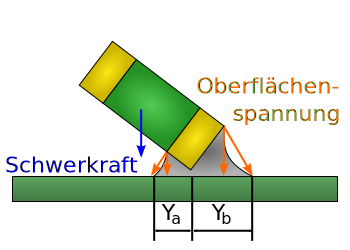
\includegraphics[width=.5\linewidth]{images/technische_grundlagen/grabsteinEffekt.png}%https://upload.wikimedia.org/wikipedia/commons/9/97/Tombstone_Effect_DE.svg
	\caption{Grabstein-Effekt \cite{wikimedia-grabstein}}
\end{figure}

\subsubsection{Popcorn-Effekt:} %aufgenommene Luftfeuchtigkeit expandiert beim Heißluftlöten und zerstört das bauteil
Ein feuchteempfindliches Bauteil, wie zum Beispiel eine Rohplatine oder das Trägermaterial eines Prozessors, welches außerhalb der vor Feuchte schützenden Verpackung gelagert wird, neigt zum Popcorn Effekt.
Das Bauteil nimmt die Feuchtigkeit aus der Umgebung auf und speichert diese.
Beim Löten verdampft das Wasser und bläht das Bauteil aufgrund der Ausdehnung auf.
Das Ausdehnen führt u. a. zu Rissen im Gehäuse oder Delaminierung der Kupferschicht.\par

Diese Fehler führen meist zur Zerstörung des Bauteils und können erst nach der Fertigung diagnostiziert werden.
Vorbeugend ist auf eine korrekte Lagerung der Komponenten zu achten.
\begin{figure}[H]
	\centering
	\includegraphics[width=.5\linewidth]{images/technische_grundlagen/popcornEffekt.jpg}%https://upload.wikimedia.org/wikipedia/commons/9/97/PopcornBGA.jpg
	\caption{Popcorn-Effekt \cite{wikimedia-popcorn}}
\end{figure}

\section{Serielle Schnittstellen}
\subsection{Universal Asynchronous Receiver/Transmitter}
\ac{uart} ist ein universell einsetzbarer elektronischer Baustein, der Systemeinheiten mit parallelem Übertragungsmodus an serielle Übertragungswege anpasst.
Mit dem \ac{uart} werden in Personal Computern (PC) die parallel anfallenden Daten in serielle Datenströme umgewandelt, die dann an den seriellen Schnittstellen (\acs{com}, \acs{lpt}, \acs{ide-drive}, usw.) für die angeschlossenen Peripheriegeräte und für die Datenübertragung über Modems zur Verfügung stehen. \cite{itwissen-uart}\par

Der \ac{uart}-Datensatz besteht aus 11 Bit, einem Startbit, acht Datenbits, einem Paritätsbit und einem Stoppbit.
Der \ac{uart} selbst besteht aus zwei \ac{fifo}-Puffern, die sende- und empfangsseitig die ein- und ausgehenden Datensignale zwischenspeichern.
Je nach Breite des Datenbusses gibt es Wandler für 8-Bit und 16-Bit mit Übertragungsraten von 19,2 kbit/s, 56 kbit/s (\ac{uart}16450) und 128 kbit/s (\ac{uart}16650D). \cite{itwissen-uart}\par
\begin{figure}[H]
	\centering
	\includegraphics[width=.9\linewidth]{images/technische_grundlagen/tide_uart_data.png}
	\caption{Aufbau eines \ac{uart}-Frames \cite{tibbo-uart}}
\end{figure}

\ac{uart} wurde für diese Anwendung ausgewählt, wegen der Einfachheit der Verdrahtung.
Die Kommunikation der Geräte findet über nur zwei Datenleitungen statt, dadurch werden Verbindungen zwischen der Platine und dem \ac{rpi} eingespart.
\ac{uart} wird vom \ac{rpi} und Mikrocontroller unterstützt.


\subsection{Serial Peripheral Interface}
Das Serial Peripheral Interface, kurz \ac{spi} oder auch Micro Wire genannt, ist ein Bussystem bestehend aus drei Leitungen für eine serielle synchrone Datenübertragung zwischen verschiedenen \acp{ic}. \cite{mikrocontroller-spi}\par

Der Bus besteht aus folgenden Leitungen
\begin{itemize}
	\item \ac{mosi}
	\item \ac{miso}
	\item \ac{sck} - Schiebetakt	
\end{itemize}
\cite{mikrocontroller-spi}

Zusätzlich zu diesen drei Leitungen wird für jeden Slave eine \ac{ss} genannte Leitung benötigt, durch die der Master den Slave zur aktuellen Kommunikation selektiert. Dies geschieht dadurch, dass der Master die \ac{ss}-Leitung von High nach Low zieht. Oft ist mit dieser Aktivierung durch den Master auch eine Benachrichtigung für den Slave verbunden mit der ihm mitgeteilt wird, dass jetzt eine Nachricht beginnt, das nächste Byte also zum Beispiel als Kommando aufzufassen ist. \cite{mikrocontroller-spi}\par

Die Übertragung geschieht so, dass der Master seine Datenleitung (\ac{mosi}) auf den Pegel des nächsten Bits bringt und dann an der \ac{sck} Leitung einen Puls ausgibt. Gleichzeitig wird vom Master der Pegel an der Datenleitung vom Slave zum Master überwacht und ihr Zustand als nächstes einzulesendes Bit aufgefasst. Üblicherweise gibt es zumindest beim Master mehrere Einstellungen, die festlegen, welches der Grundzustand dieser \ac{sck} Leitung sein soll und welche Flanke des Taktes zur Datenübernahme herzunehmen ist (die steigende oder die fallende). Bei einigen Slaves ist diese Einstellung ebenfalls möglich, oft ist es aber so, dass per \ac{spi} anzusprechende \ac{ic} eine feste Einstellung benutzen, an die sich der Master anpassen muss. \cite{mikrocontroller-spi}\par

Für den \ac{spi}-Bus gibt es kein festgelegtes Protokoll. Die Taktpolarität und Phase können ebenfalls von Slave zu Slave unterschiedlich sein. Der \ac{spi}-Bus kann mit einer Taktfrequenz von vielen Megahertz betrieben werden. Es gibt viele verschiedene \acp{ic} die als Slave an dem \ac{spi}-Bus betrieben werden können, diese gehen von einfachen Schieberegistern bis hin zu \acp{rtc} oder Displaytreibern mit vorgegebenem Protokoll. Unter anderem werden die meisten AVR-Microcontroller von Atmel über \ac{spi} programmiert. \cite{mikrocontroller-spi}\par

\section{Audio-Verstärker Class D}
Mit Class-D wird ein bestimmtes Schaltungsdesign von Audio-Verstärkern bezeichnet, die ein \ac{pwm}-Signal erzeugen und daher auch als \ac{pwm}-Verstärker bekannt sind. \cite{fairaudio-classd}\par

Es hat sich vielerorts heute eingebürgert, „Class-D“ mit „digital“ zu übersetzen. Historisch war „D“ jedoch als Kategorie an der Reihe, nachdem die Buchstaben „A“, „B“ und „C“ bereits für andere Verstärkerklassen vergeben waren, die früher aufkamen. Heute nutzen einige Class-D-Designs intern auch Digitaltechnik. Dies kann durch die Zusatzeigenschaft „digitally controlled“ (digital kontrolliert) ausgedrückt werden. Das \ac{pwm}-Signal am Verstärkerausgang ist dabei in jedem Fall als ein Analogsignal zu sehen, welches nach Tiefpassfilterung direkt zur Ansteuerung eines Lautsprechers verwendet werden kann. \cite{fairaudio-classd}\par

Da auch von Schaltverstärkern gesprochen wird und tatsächlich die Ausgangsstufe entweder „An“ oder „Aus“ ist, liegt die vereinfachende Analogie zur Digitaltechnik aber nahe: Bei dieser wird ebenfalls mit binären Werten (0/1 – Aus/An) gearbeitet (dazu weiter unten mehr). Ein wesentliches Merkmal der Digitaltechnik – die festgelegte Anzahl von Stufen bei Fehlen von Zwischenwerten (die Wortbreite, z. B. 16 Bit) – gibt es bei Class-D-Schaltungen aber nicht. Bei ihr sind (zumindest theoretisch) unendlich viele Zwischenstufen möglich, auch wenn in der Praxis sicherlich Restriktionen auftreten. \cite{fairaudio-classd}\par

Eine Class-D Schaltung lässt sich schematisch in drei Bereiche unterteilen:
\begin{enumerate}
	\item Der erste Bereich besteht aus dem Eingang für das Audiosignal, einem Signal-Generator (Dreieck) und einem sogenannten Komparator (Comp).
	\item Die eigentliche Schalt-Verstärkungsstufe enthält einen Controller und die Transistoren, die das vom Komparator kommende \ac{pwm}-Signal verstärken.
	\item Das Tiefpass-Filter (hohe Frequenzen werden herausgefiltert), welches das am Eingang generierte Signal (die Trägerfrequenz) wieder herausfiltert.	
\end{enumerate}
\cite{fairaudio-classd}
\begin{figure}[H]
	\centering
	\includegraphics[width=.9\linewidth]{images/technische_grundlagen/class-d-schematisch.png}
	\caption{Schematische Darstellung Class-D \cite{fairaudio-classd}}
\end{figure}
%falls noch mehr text benötigt wird: erklärungen auf website
\chapter{Berechnung}
\wip
\section{Spannungsabfall}
Herkömmliche Cat5-Ethernetkabel wurden ursprünglich nicht für die Übertragung großer elektrischer Leistungen entwickelt und besitzen daher Leitungen mit einem sehr geringen Ader-Durchmesser.
Aufgrund dieser Gegebenheit kann es bei weiten Entfernungen oder großen übertragenen Leistungen zu abnormal hohen Spannungsabfällen kommen.
Um die Anlage in dieser Hinsicht zu überprüfen werden sämtliche Spannungsabfälle und die damit verbundenen Verlustleistungen bei maximaler Belastung durch die Stationen berechnet.
Zur Berechnung der Spannungsabfälle sind folgende Angaben verwendet worden.
\begin{itemize}
	\item Es werden vier Stationen über \ac{poe} versorgt.
	Die Stationen sind nach Abbildung \crossref{fig:poe-verdrahtung} miteinander verdrahtet.
	\item Jede Station hat einen maximalen Leistungsverbrauch von 12 W.
	\item Das Ethernetkabel zwischen den Stationen hat jeweils eine Länge von 10 m.
	\item Der Querschnitt einer Ader des Ethernet-Kabels beträgt 0.128 mm\textsuperscript{2} \cite[vgl.][]{lapp-cat5-datasheet}.
	\item Am \ac{pse} wird eine Spannung von 30 V in das Netz eingespeist.
\end{itemize}
\begin{figure}[htbp!]
	\centering
	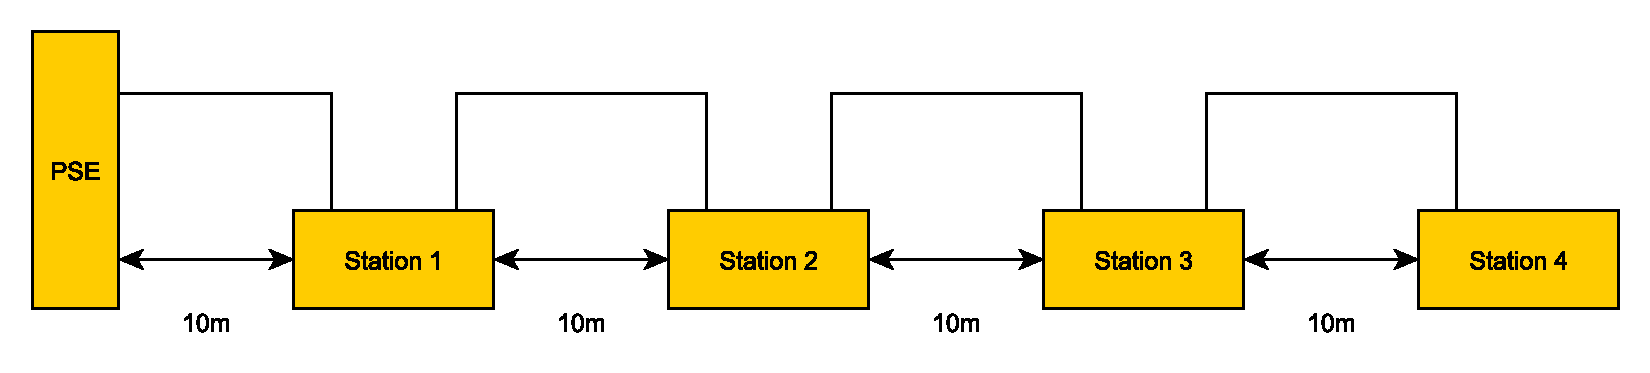
\includegraphics[width=.9\linewidth]{images/berechnung/poe_verdrahtung.png}
	\caption{Verdrahtungsschema}
	\label{fig:poe-verdrahtung}
\end{figure}
Der Leitungswiderstand eines Adernpaares des Ethernetkabels beträgt nach der allgemeinen Drahtwiderstandsformel $R_{Ltg}=\frac{l}{\gamma\cdot A}=0.686\Omega$.
Bei den \ac{poe}-Typen 1 und 2 wird je ein Adernpaar für die Zu- und Rückleitung verwendet.
Bei den \ac{poe}-Typen 3 und 4 werden je zwei Adernpaare parallel geschaltet.\par

Daraus ergeben sich die in den Abbildungen \ref{fig:ers-type12} und \ref{fig:ers-type34} dargestellten Ersatzschaltungen.
Die Stationen (Verbraucher) sind als Widerstand gezeichnet, wobei sie sich nicht wie ein solcher verhalten.
\begin{figure}[htbp!]
	\centering
	\includegraphics[width=\linewidth]{images/berechnung/poe2pair.png}
	\caption{Ersatzschaltung  \ac{poe} Type 1 und 2}
	\label{fig:ers-type12}
\end{figure}
\begin{figure}[htbp!]
	\centering
	\includegraphics[width=\linewidth]{images/berechnung/poe4pair_neu.jpg}
	\caption{Ersatzschaltung  \ac{poe} Type 3 und 4}
	\label{fig:ers-type34}
\end{figure}

Anhand der in den Abbildungen \ref{fig:ers-type12} und \ref{fig:ers-type34} dargestellten Ersatzschaltungen ergibt sich ein Gleichungssystem in 8 Variablen. Die Quellenspannung ist mit U\textsubscript{0} bezeichnet, der Strom und die Spannung der Station n mit I\textsubscript{n} bzw. U\textsubscript{n}.
\begin{align}
	U_1 &= U_0-2\cdot R_{Ltg}\cdot (I_1+I_2+I_3+I_4)\\
	U_2 &= U_1-2\cdot R_{Ltg}\cdot (I_2+I_3+I_4)\\
	U_3 &= U_2-2\cdot R_{Ltg}\cdot (I_3+I_4)\\
	U_4 &= U_3-2\cdot R_{Ltg}\cdot I_4\\
	12W &= U_1\cdot I_1\\
	12W &= U_2\cdot I_2\\
	12W &= U_3\cdot I_3\\
	12W &= U_4\cdot I_4
\end{align}

Dieses Gleichungssystem von Hand zu lösen, würde viel Zeit in Anspruch nehmen.
Daher wurde für die Lösung auf das Computerprogramm wxMaxima zurückgegriffen.
Die Eingabe der Gleichungen erfolgt in Textform (siehe Abbildung \ref{fig:maxima-input})\par

wxMaxima ist eine dokumentenbasierte Schnittstelle für das Computeralgebrasystem Maxima. wxMaxima bietet Menüs und Dialoge für viele gängige Maxima-Befehle, Autovervollständigung, Inline-Plots und einfache Animationen. wxMaxima wird unter der \ac{gpl}-Lizenz vertrieben. \cite[aus dem Englischen übersetzt]{wxmaxima}\par

\begin{figure}[htbp!]
	\centering
	\includegraphics[width=.9\linewidth]{images/berechnung/max_2pair_30V.png}
	\caption{Eingabe wxMaxima Type 1 \& 2}
	\label{fig:maxima-input}
\end{figure}

Die Lösungen für das Gleichungssystem werden vom Programm in Textform zurückgegeben.
Das Programm findet neben der relevanten Lösung noch einige komplexe Lösungen für das Gleichungssystem.
Diese werden hier wegen Platzgründen und niedriger Relevanz weggelassen.
\begin{table}[H]
	\centering
	\begin{tabular}{r|ccc|ccc}
		\toprule
		&\multicolumn{3}{c|}{Type 1 \& 2}&\multicolumn{3}{c}{Type 3 \& 4}\\\cmidrule{2-7}
		&U&\tdelta U&I&U&\tdelta U&I\\
		\midrule
		Quelle&30.00 V&&1931 mA&30.00 V&&1729 mA\\
		\midrule
		Station 1&27.35 V& 8.83\%&438 mA&28.81 V& 3.97\%&416 mA\\
		Station 2&25.30 V&15.67\%&474 mA&27.91 V& 6.97\%&430 mA\\
		Station 3&23.90 V&20.33\%&502 mA&27.31 V& 8.97\%&439 mA\\
		Station 4&23.19 V&22.70\%&517 mA&27.00 V&10.00\%&444 mA\\
		\bottomrule
	\end{tabular}
	\caption{Berechnung Ergebnisse}
\end{table}
Bei einer Quellenspannung von 30 V und einem Gesamtstrom von 1.931 A (Type 1 \& 2) bzw. 1.729 A (Type 3 \& 4) ergibt sich eine Gesamtleistung von 57.93 bzw. 51.87 W.
Bei Type 3 \& 4 ist die Belastung der Quelle um 10 \% niedriger als bei Type 1 \& 2.

Man sieht: Der Spannungsabfall ist wie erwartet bei Type 3 und 4 weniger als halb so groß wie bei Type 1 und 2.
Dadurch ist auch die gesamte Verlustleistung der Leitungen geringer, was eine niedrigere Belastung der Quelle bedeutet.

Aus der obigen Rechnung ergibt sich, dass für die gegebene Anlage eine Versorgung nach Type 3 bzw. 4 empfehlenswert ist.
\chapter{Verbesserte Hardwarelösung}
\section{Konzept}
Die neue Lösung sollte den Aufbau einer Station vereinfachen und die Ausfallsrate einer Station auf gänzlich null reduzieren.
Um dieses Ziel zu erreichen, werden folgende Ansätze definiert:

\paragraph{Zusammenfassen der Platinen zu einer einzigen:}
Die Reduktion der Anzahl der Platinen auf eine Platine ermöglicht die Zusammenfassung von verschiedenen Modulen.
Damit werden die Produktionskosten gesenkt und die Montage in den Stationen vereinfacht.

\paragraph{Reduzierung der Bauteile:}
Die Zusammenfassung der Module auf eine einzelne Platine ermöglicht die Reduktion von Bauteilen.
Insbesondere werden Bauteile für die Verbindungstechnik eingespart.
Dies führt zu einer Kostenreduktion bei gleichzeitiger Senkung der Fehlermöglichkeiten. 

\paragraph{Entfall der Verdrahtung zwischen den Einzelplatinen:}
Der Entfall der Verdrahtung führt zu einer Steigerung der Übersichtlichkeit und reduziert zusätzlich den Platzbedarf.
Aufwände für die händische Verdrahtung und die Prüfung der Verbindungen der einzelnen Platinen entfällt.
Fehlverdrahtung wird konstruktiv durch die Einzelplatine verhindert.

\paragraph{Verbesserung der Spannungsversorgung:}
Leistungsbeschränkungen sowie die Verwendung eines neuen verbesserten Spannungsreglers verbessern die Spannungsqualität.
Die verstärkte Spannungsversorgung ermöglicht ein späteres Update auf den leistungsstärkeren \ac{rpi} Model 4.

\paragraph{Einführung WatchDogTimer:}
Zusätzlich wird ein Watchdog mittels eines Mikroprozessors verbaut.
Dieser wird benötigt, um eventuelle Ausfälle des \ac{rpi} und somit der gesamten Station zu erkennen.
Falls ein Fehler auftritt, setzt der Mikroprozessor den \ac{rpi} zurück und die Station startet neu.
Nachdem die Station neugestartet ist, wird der Normalbetrieb wieder aufgenommen und der Watchdog nimmt den Zustand des Überwachens wieder ein.

%Lösungen für probleme, zusätzliche vorteile
\section{Spannungsversorgung}
\subsection{Anforderungen}
Um einen möglichst reibungslosen Betrieb zu garantieren, werden an die Spannungsversorgung mehrere Anforderungen gestellt:
\begin{itemize}
	\item Der Eingangsspannungsbereich muss mindestens 24 bis 35 V betragen.
	\item Die gewünschte Ausgangsspannung beträgt 5 V.
	\item Der Oberwellenanteil (ripple) der Ausgangsspannung soll unter 1\% liegen. 
	\item Die Strombelastbarkeit muss mindestens 2.5 A betragen.
\end{itemize}
Die Versorgungsspannung wird über  \ac{poe} (Power over Ethernet) zur Verfügung gestellt.
Der Spannungsregler muss diese Art der Versorgungsspannung unterstützen.
Der Spannungsregler sollte die 24 V auf 5 V möglichst verlustarm reduzieren.
Alle versorgten Komponenten auf der Platine arbeiten mit einer Spannung von 5 V.
Diese Komponenten sind z.B. der \ac{rpi}, der Mikrocontroller und die Verstärkerschaltung für Mikrofon und Lautsprecher.\par

Die Spannungsversorgung soll bei Spannungsschwankungen kurzzeitig die Versorgung aufrechterhalten, um dem Versagen einer Station vorzubeugen.
Zur Stützung der Spannungsversorgung werden Kondensatoren auf der Eingangsspannungsseite und auf der Ausgangsspannungsseite benötigt.

\subsection{Auswahl Spannungsregler}
Aufgrund der oben angeführten Anforderungen wird der Spannungsregler LM33630 ausgewählt.
Dieser Spannungsregler kann im Bereich von 3.8 V bis 36 V betrieben werden.
Die Ausgangsspannung ist immer kleiner als die Eingangsspannung und liegt im Bereich von 1 V bis 24 V.
Der LM33630 ist ein Step-down Spannungsregler, das bedeutet er kann nur von einer höheren auf eine niedrigere Spannung regeln.\par

Um eine Schwingung, die wenig Aufwand zur Glättung benötigt, zu erzeugen, verwendet der Spannungsregler eine hohe Schaltfrequenz von 2.1 MHz.
Der LM33630 hat standardmäßig einen maximalen Ausgangsstrom von 3 A, dieser wird auch nahezu vollständig benötigt für den \ac{rpi}, der allein bereits ca. 1.5 A bezieht.
Der Lautsprecher mit der Vorschaltung benötigt ebenfalls über 0.5 A.\par

Vom LM33630 sind mehrere Varianten verfügbar, es gibt die DDA und RNX Variante.
Die DDA Variante hat 8 Pins und einen eingebauten Kühlkörper, der mit einem großen Massefeld verbunden werden kann, damit der \ac{ic} nicht überhitzt.
Die RNX Variante hat 12 Pins und anstatt eines größeren Kühlfläche mehrere Ground Pins, die ebenfalls zur Kühlung des \ac{ic} dienen.
Zusätzlich gibt es eine weitere Unterteilung der zwei Varianten: es gibt verschiedene Schaltfrequenzen, nämlich 400, 1400 und 2100 kHz.\par
Die technischen Daten dieses Spannungsreglers sind in vollem Umfang im Datenblatt ersichtlich. \cite[vgl.][]{lmr33630-datasheet}

\subsection{Funktion des Spannungsreglers}
Der hier gewählte Spannungsregler ist ein Schaltregler, d.h. er verändert den Effektivwert der Spannung mit \ac{pwm}.
Über einen Spannungsteiler kann die gewünschte Ausgangsspannung eingestellt werden.
Weiters kann der Spannungsregler abgeschaltet werden, wenn 0 V am Enable Pin angelegt werden.
Dies sorgt für eine komplette Abschaltung der Steuerlogik.
Die Verwendung dieser Funktion ist jedoch nicht vorgesehen.

\subsection{Zusatzbeschaltung des Spannungsreglers}
Der Spannungsregler ist universell einsetzbar, weshalb die genauen Betriebseigenschaften über die externe Beschaltung festgelegt werden.
\paragraph{Eingangskondensator:}
Auf der Eingangsseite, d.h. der 24 V Seite wird ein 820 µF Kondensator verbaut.
Dieser dient in erster Linie zum Abfangen und Ausgleichen von Spannungsschwankungen.
Diese Spannungsschwankungen können aufgrund von sich schlagartig änderndem Leistungsverbrauch entstehen.

\paragraph{Ausgangskondensator:}
Nach dem Spannungsregler auf der 5 V Seite werden zwei Kondensatoren mit jeweils der Kapazität von 1 mF verbaut, das ergibt eine Gesamtkapazität auf der 5 V Seite von 2 mF.
Diese werden zur nahezu vollständigen Glättung der Ausgangsspannung und weiteres Abfangen von Spannungseinbrüchen aufgrund von Leistungsspitzen verwendet.

\paragraph{Spannungsteiler:}
Der Spannungsteiler (100 kOhm; 23,9 kOhm) am FB Pin sorgt für die richtige Ausgangsspannung von 5 V.
Dieser Spannungsteiler kann frei über die folgende Formel konfiguriert werden:
\[R_{FBB}=\frac{R_{FBT}}{\frac{V_{OUT}}{V_{REF}}-1}\]
Im Datenblatt des Spannungsreglers sind bereits Werte für die am häufigsten verwendeten Spannungen vorgegeben.

\paragraph{Kühlung:}
Der Spannungsregler muss gekühlt werden, da bei ihm eine nicht vernachlässigbare Verlustleistung auftritt.
Unter dem \ac{ic} ist eine große Massenfläche bereitgestellt, die zur Kühlung dient.
Die Kühlfläche des Spannungsreglers wird mit Durchkontaktierungen (Vias) mit der Massefläche auf der Unterseite der Platine verbunden und somit gekühlt.

\section{Lautsprecher-Verstärker}
Ein Audio-Leistungsverstärker (oder Leistungsverstärker) ist ein elektronischer Verstärker, der elektronische Audiosignale mit geringer Leistung, wie z.B. das Signal von einem Radioempfänger oder einem E-Gitarren-Tonabnehmer, auf einen Pegel verstärkt, der hoch genug ist, um Lautsprecher oder Kopfhörer anzutreiben.
Während das Eingangssignal eines Audio-Leistungsverstärkers, wie z.B. das Signal einer elektrischen Gitarre, vielleicht nur einige hundert Mikrowatt misst, kann seine Ausgangsleistung bei kleinen Geräten der Unterhaltungselektronik, wie z.B. Radiowecker, einige zehn oder hundert Watt für eine Heimstereoanlage, mehrere tausend Watt für die Beschallungsanlage eines Nachtclubs oder Zehntausende von Watt für ein großes Rockkonzert-Soundsystem betragen. \cite[vgl.][]{electronicshub-pwm-amp}

\subsection{Anforderungen}
Wichtige Entwurfsparameter für Audio-Leistungsverstärker sind Frequenzgang, Verstärkung, Rauschen und Verzerrung.
Diese sind voneinander abhängig; eine Erhöhung der Verstärkung führt oft zu einer unerwünschten Zunahme von Rauschen und Verzerrung.
Eine negative Rückkopplung reduziert zwar die Verstärkung, aber auch die Verzerrung.
Der Verstärkerchip soll einen Lautsprecher mit 8 \tOmega\ betreiben können.
Er sollte eine Leistung aufweisen, damit die Töne beim Lautsprecher ausreichend laut abgespielt werden.
Der Lautsprecherverstärker soll einen möglichst hohen Wirkungsgrad besitzen, um die Verlustleistung möglichst niedrig zu halten und damit zusätzliche Kühlung zu vermeiden.

\subsection{Auswahl}
Der PAM8403 ist ein 3W, Klasse-D-Audioverstärker. Er bietet einen niedrigen THD+N-Wert (bedeutet „total harmonic distortion plus noise“.
Sie wird normalerweise, durch Eingabe einer Sinuswelle, Bandsperrfilterung des Ausgangs und Vergleich des Verhältnisses zwischen dem Ausgangssignal mit und ohne Sinuswelle, gemessen), wodurch eine hochwertige Klangwiedergabe erreicht wird. 
Die neue filterlose Architektur ermöglicht es dem Gerät, den Lautsprecher direkt anzusteuern, so dass keine Tiefpassausgangsfilter erforderlich sind, wodurch Systemkosten und Leiterplattenfläche eingespart werden.
Der PAM8403 weist eine Effizient von bis zu 90 \% auf, deutlich höher als Verstärker aus den anderen Verstärkerklassen.
Diese weisen in den niederen Leistungsbereich meist eine Effizient von 50 \% auf.
Bei einem 8 \tOmega\ Lautsprecher ist eine maximale Leistung von 1.5 W möglich und ein Wirkungsgrad von 90 \%.

\subsection{Funktionen}
\paragraph{Maximale Verstärkung:}
Der PAM8403 hat zwei interne Verstärkerstufen.
Die Verstärkung der ersten Stufe ist extern konfigurierbar, während die der zweiten Stufe intern fest eingestellt ist.
Die Regelverstärkung der ersten Stufe wird durch die Wahl des Verhältnisses von RF zu RI eingestellt, während die Verstärkung der zweiten Stufe auf 2x festgelegt ist.
Der Ausgang von Verstärker 1 dient als Eingang zu Verstärker 2, sodass die beiden Verstärker Signale erzeugen, die in der Größe identisch sind, sich aber in der Phase um 180° unterscheiden.

\paragraph{Mute Funktion:}
Der MUTE-Pin ist ein Eingang zur Steuerung des Ausgangszustandes des PAM8403.
Ein logisches Low an diesem Pin deaktiviert die Ausgänge, und ein logisches High an diesem Pin aktiviert die Ausgänge.
Dieser Pin kann als schnelle Deaktivierung oder Aktivierung der Ausgänge ohne Lautstärkeschwund verwendet werden.
Der MUTE-Pin kann aufgrund des internen Pull-ups potentialfrei bleiben.

\paragraph{Shutdown Funktion:}
Um den Stromverbrauch bei Nichtbenutzung zu reduzieren, enthält der PAM8403 eine Abschaltung, mit der die Vorspannungsschaltung des Verstärkers abgeschaltet werden kann.
Diese Abschaltfunktion schaltet den Verstärker ab, wenn am SHDN-Pin ein logischer Low-Wert anliegt.
Durch Schalten des mit GND verbundenen SHDN-Pins wird die Stromaufnahme des PAM8403 im Leerlauf minimiert.
Der SHDN-Pin kann aufgrund des internen Pull-ups potentialfrei bleiben.

\subsection{Zusatzbeschaltung}
Der Verstärker benötigt nur wenige Komponenten als Zusatzbeschaltung.
Die Spannungsversorgung wird mit Kondensatoren parallelgeschaltet, um mögliche Spannungsschwankungen auszugleichen.
Der Eingang des Audiosignales vom \ac{rpi} wird zuerst über einen Kondensator geführt um Störungen zu vermeiden und Gleichanteile herauszufiltern.\par

Der Audioverstärker hat insgesamt 3 Masseanschlüsse, darunter befindet sich ein Masseanschluss für die interne Steuerschaltung.
Die zwei anderen Pins sind für die zwei Lautsprecher selbst, über sie fließt der Strom des Lautsprechers ab.

\subsection{Kühlung}
Der Audioverstärker muss nicht aktiv gekühlt werden, da ein Wirkungsgrad von rund 90 \% vorliegt.
Das bedeutet bei einer Leistung von 1.5 W tritt nur eine Verlustleistung 0.15 W auf.

\section{Mikrocontroller}
Ein Mikrocontroller ist ein Halbleiterchip, der einen Prozessor und zugleich auch Peripheriefunktionen enthält.
Der Arbeits- und Programmspeicher befindet sich vollständig auf demselben Chip, deshalb ist der Mikrocontroller ein Ein-Chip-Computersystem.
Auf modernen Controllern finden sich auch komplexe Peripheriefunktionen, sowie die Schnittstellen \ac{usb}, \ac{i2c} und \ac{spi}, \ac{pwm}-Ausgänge oder Analog-Digital-Umsetzer.
Es gibt eine breite Menge an verschiedenen Mikrocontrollern.
Angefangen bei Controllern mit einem Takt von 4 kHz und Leistung von wenigen Milliwatt oder Mikrowatt für einfache Aufgaben, wie Warten auf Betätigen eines Tasters.
Bis zu Controllern mit einem Takt von mehrere MHz und einen Programmspeicher von mehreren kBytes für größere und komplexere Aufgaben.\par

Der AVR-Mikrocontroller ATmega328P wurde aus mehreren Gründen ausgewählt:
\begin{itemize}
	\item Das Programmieren dieses Chips wird einerseits durch die Unterstützung der Arduino \ac{ide-dev}, mit der wir bereits sehr gut vertraut sind, sehr stark vereinfacht.
	\item Das Hochladen des Programmes in den ATmega328P stellt ebenfalls kein Problem dar, ein Arduino kann als \ac{icsp} verwendet werden.
	\item Der Controller benötigt nur eine minimale Beschaltung, um ordnungsgemäß zu funktionieren.
\end{itemize}

\subsection{Atmel AVR}
Die AVR-Mikrocontroller von Atmel (jetzt Microchip Technology Inc.) sind wegen ihrer übersichtlichen internen Struktur, der In-System-Programmierbarkeit, und der Vielzahl von kostenlosen Programmen zur Softwareentwicklung (Assembler, Compiler) beliebt. Diese Eigenschaften und der Umstand, dass viele Typen in einfach handhabbaren \ac{dip}-Gehäusen verfügbar sind, machen den AVR zum idealen Mikrocontroller für Anfänger.
Über die Bedeutung des Namens \enquote{AVR} gibt es verschiedene Ansichten; manche meinen es sei eine Abkürzung für Advanced Virtual \ac{risc}, andere vermuten dass der Name aus den Anfangsbuchstaben der Namen der Entwickler (Alf Egil Bogen und Vegard Wollan \ac{risc}) zusammengesetzt wurde. Laut Atmel ist der Name bedeutungslos.

\subsection{Architektur}
Die Architektur ist eine 8-Bit-Harvard-Architektur, das heißt, es gibt getrennte Busse zum Programmspeicher (Flash-ROM, dieser ist 16 bit breit) und Schreib-Lese-Speicher (RAM). Der Programmcode kann ausschließlich aus dem Programmspeicher ausgeführt werden. Weiterhin sind die Adressräume unabhängig (d.h. beide Speicher besitzen eigene Adressbereiche, die sich wertemäßig überschneiden können). Bei der Programmierung in Assembler und einigen C-Compilern bedeutet dies, dass sich Konstanten aus dem ROM nicht mit dem gleichen Code laden lassen wie Daten aus dem RAM. Abgesehen davon ist der Aufbau des Controllers recht übersichtlich und birgt wenige Fallstricke.
\begin{itemize}
\item 32 größtenteils gleichwertige Register
\item davon 1–3 16-bit-Zeigerregister (paarweise)
\item ca. 110 Befehle, die meist 1–2 Taktzyklen dauern
\item Taktfrequenz bis 32 MHz
\item Betriebsspannung von 1,8 – 5,5 V
\item Speicher (1-256 kB Flash-ROM, 0-4 kB EEPROM, 0-16 kB RAM)
\item Peripherie: Analog-Digital-Wandler 10 Bit, 8- und 16-Bit-Timer mit \ac{pwm}, \ac{spi}, \ac{i2c}, \ac{uart}, Analog-Komparator, Watchdog
\item 64 kB externer SRAM (ATmega128, ATmega64, ATmega8515/162)
\item JTAG bei den größeren ATmegas
\item debugWire bei den neueren AVRs		
\end{itemize}
\cite[Architektur]{mikrocontroller-avr}

\subsection{Funktion}
Der Mikrocontroller übernimmt in diesem Projekt mehrere Aufgaben.
\subsubsection{Watchdog-Timer für Raspberry Pi}
Ein Watchdog-Timer überwacht, ob ein System noch funktionsfähig ist, oder ob es irgendwo festhängt.
In letzterem Fall wird vom Watchdog-Timer in den meisten Anwendungen ein Hardware-Reset ausgelöst.\par

Der Mikrocontroller kommuniziert periodisch mit dem \ac{rpi} über \ac{uart}, d.h. der Mikrocontroller sendet eine Nachricht und der \ac{rpi} schickt eine Antwort zurück.
Wenn die Antwort des \ac{rpi} ausbleibt, hat sich dieser offensichtlich aufgehängt und muss zurückgesetzt werden.
Der Mikrocontroller setzt den Reset-Pin des \ac{rpi} auf Low und erzwingt damit einen Neustart der Station.
Nachdem der \ac{rpi} neugestartet ist, meldet er dies dem Mikrocontroller.
Der Mikrocontroller geht wieder in den Zustand des Überwachens über und der \ac{rpi} setzt seine normale Funktion fort.

\subsubsection{IO-Handling}
Über den Mikrocontroller werden sämtliche digitale Eingänge aufgenommen und an den \ac{rpi} weitergegeben.
Dies ist für die Diebstahlsicherung der Außenstation essenziell.
Weiters steuert der \ac{rpi} über die Digital-Ausgänge des Mikrocontrollers den Audio-Verstärker-\ac{ic} hinsichtlich Betrieb an.

\subsection{Zusatzbeschaltung}
\paragraph{Reset-Pin:}
Der Reset Pin des Mikrocontroller ist bei einer Spannung von 0 V aktiv.
Damit er im normalen Betrieb nicht aktiviert wird, wird er über einen Widerstand auf 5 V gezogen.
Um den Reset Pin nun zu aktivieren, muss nur zwischen dem Widerstand und dem Reset Pin 0 V angelegt werden.
Damit verändert sich das Potential des Reset Pin auf 0 V und wird aktiviert.

\paragraph{Clock:}
Die Clock des Mikrocontrollers wird durch einen Schwingquarz erzeugt.
Ein Schwingquarz, häufig vereinfachend abgekürzt als Quarz bezeichnet, ist ein elektronisches Bauelement, welches zur Erzeugung von elektrischen Schwingungen mit einer bestimmten Frequenz dient.
Über die Schwingfrequenz wird die Arbeitsgeschwindigkeit des Mikrocontrollers festgelegt.
In diesem Fall wird ein Quartz mit 6 MHz verwendet.
\chapter{Hardware-Programmierung}
\section{Programm-Entwicklung}
Die für diese Diplomarbeit entwickelte Hardware enthält intelligente Komponenten, die auch programmiert werden müssen.
Diese sind zum einen der bereits vorher existierende \ac{rpi} und der neu hinzugefügte ATmega328P Mikrocontroller.
\subsection{Mikrocontroller}
\subsubsection{Entwicklungsumgebung}
Die \ac{ide-dev} von Arduino ist eine plattformübergreifende Anwendung (für Windows, MacOS, Linux), die in Funktionen aus C und C++ geschrieben ist.
Sie wird zum Schreiben und Hochladen von Programmen auf Arduino-kompatible Boards, aber auch, mit Hilfe von 3rd-Party-Cores, auf Entwicklungsboards anderer Hersteller verwendet.

Der Quellcode für die \ac{ide-dev} wurde unter der GNU \ac{gpl} Version 2, veröffentlicht.
Die Arduino \ac{ide-dev} unterstützt die Sprachen C und C++ unter Verwendung spezieller Regeln der Code-Strukturierung.
Die Arduino \ac{ide-dev} liefert eine Software-Bibliothek aus dem Wiring-Projekt, die viele gängige Ein- und Ausgabeprozeduren zur Verfügung stellt.
Der benutzergeschriebene Code benötigt nur zwei grundlegende Funktionen, \texttt{setup()} zum Starten des Sketch und der Hauptprogrammschleife \texttt{loop()}, die kompiliert und mit einem Programmstub \texttt{main()} zu einem ausführbaren zyklischen Ausführungsprogramm mit der GNU-Toolchain, die ebenfalls in der \ac{ide-dev}-Distribution enthalten ist, verknüpft werden.
%quelle!!

\subsubsection{Programmierung}
Der in dieser Diplomarbeit verwendete Mikrocontroller besitzt keine \ac{usb}-Schnittstelle, sondern muss über ein externes Programmiergerät mittels \ac{spi}-Schnittstelle programmiert werden.

Als Programmiergerät wurde ein Arduino-Mega-Entwicklungsboard gewählt. Dieses verfügt über eine \ac{icsp}-Schnittstelle, mit der ein anderer Mikrocontroller über \ac{spi} programmiert werden kann. Diese Schnittstelle und deren Pinbelegung ist in Abbildung \ref{fig:icsp-header} dargestellt.
\begin{figure}[htbp!]
    \centering
    \includegraphics[width=8cm]{images/hardware-programmierung/ICSPHeader.jpg}
    \caption[\ac{icsp} Schnittstelle \cite{arduino-isp}]
            {\ac{icsp} Schnittstelle \cite[How to wire your boards]{arduino-isp}}
    \label{fig:icsp-header}
\end{figure}

Das Arduino-Board, welches als Programmiergerät verwendet wird, muss mit Hilfe des mitgelieferten Programmes als \ac{isp}-Programmiergerät konfiguriert werden. Das Programm ist in der Arduino \ac{ide-dev}, wie in Abbildung \ref{fig:arduino-isp-sketch} dargestellt, zu finden.
\begin{figure}[htbp!]
    \centering
    \includegraphics[width=.9\linewidth]{images/hardware-programmierung/arduino-isp-sketch.png}
    \caption{ArduinoISP Sketch}
    \label{fig:arduino-isp-sketch}
\end{figure}

Bevor das eigentliche Programm auf den Mikrocontroller der Station hochgeladen werden kann, müssen noch ein paar Einstellungen in der Arduino \ac{ide-dev} getroffen werden (siehe auch Abbildung \ref{fig:arduino-options}):
\begin{itemize}
    \item Arduino/Genuino Uno als Board auswählen (Dieses Board wird standardmäßig mit dem hier verwendeten Mikrocontroller ausgeführt)
    \item Auswahl der Schnittstelle, an welche das Programmiergerät angeschlossen ist.
    \item Die Option \enquote{Programmer} muss von \enquote{AVRISP mkII} auf \enquote{Arduino as ISP} umgestellt werden.
\end{itemize}
\begin{figure}[htbp!]
    \centering
    \includegraphics[width=.9\linewidth]{images/hardware-programmierung/optionen.png}
    \caption{Arduino \ac{ide-dev} Einstellungen}
    \label{fig:arduino-options}
\end{figure}

Um nun den Upload-Prozess zu starten muss in der Arduino \ac{ide-dev} \enquote{Upload using Programmer} ausgewählt werden (siehe Abbildung \ref{fig:arduino-upload}).
Das Mikrocontroller-Programm wird nun kompiliert und mit Hilfe des Programmiergerätes auf den Mikrocontroller geladen.
\begin{figure}[htbp!]
    \centering
\includegraphics[width=.7\linewidth]{images/hardware-programmierung/upload.png}
    \caption{Hochladen des Programmes}
    \label{fig:arduino-upload}
\end{figure}

\subsubsection{Programm-Dokumentation}
Der Mikrocontroller wird in C++ mit vorgefertigten Funktionen von Arduino programmiert.

\begin{minted}[firstnumber=1]{arduino}
#include <TimerOne.h>
const int ResetPin = 2, MutePin = 3, SecurityPin = 4;
volatile bool FindEnable = false;
bool Reboot = true;
\end{minted}
\paragraph{1:}
Die TimerOne Bibliothek ermöglicht die Verwendung der Intrerrupt-Funktion des Hardware-Timers des Mikrocontrollers, wodurch das periodische Aufrufen einer Funktion vereinfacht wird.
Dies dient dem ständigen Abfragen des Betriebszustandes des \ac{rpi}.

\paragraph{2:}
Hier werden die verwendeten Pin-Nummern des Mikrocontrollers in Konstanten gespeichert, um das Programm lesbar zu halten.
Zu beachten ist, dass die Nummern des Programms nicht mit den physikalischen Pin-Nummern übereinstimmen.
Das liegt daran, dass die Zuordnung auf einem Arduino-Entwicklungs-Board basiert.

\paragraph{3-4:}
Weiters werden alle globalen Variablen definiert.
Das volatile-Schlüsselwort wird gebraucht, wenn die Variable in einer Interrupt Service Routine verändert wird.
Das Schlüsselwort hat zur Folge, dass der Wert der Variable nicht zwischengespeichert, sondern immer der aktuelle Wert abgerufen wird.
Dies ist notwendig, da die \ac{isr} den Programmablauf jederzeit unterbrechen und den Wert zu einem ungünstigen Zeitpunkt verändern kann.

\begin{minted}[firstnumber=6]{arduino}
void setup()
{
    pinMode(ResetPin, OUTPUT);
    pinMode(MutePin, OUTPUT);
    pinMode(SecurityPin, INPUT);
    
    Serial.begin(9600);
    Serial.setTimeout(1000);
    Timer1.initialize(10000000);
    Timer1.attachInterrupt(Check);
    digitalWrite(MutePin, HIGH);
}
\end{minted}
Die Setup-Funktion wird einmalig nach dem Start bzw. Reset des Mikrocontrollers aufgerufen. In dieser werden meist Initialisierungen durchgeführt.

\paragraph{8-10:}
Mit pinMode() wird festgelegt, ob ein \ac{io}-Pin als Ausgang oder als Eingang konfiguriert ist.

\paragraph{12-13:}
Die serielle \ac{uart}-Schnittstelle kann mit dem Serial-Objekt manipuliert werden.
Zum Initialisieren muss die Übertragungsrate in Bit/s angegeben werden, da \ac{uart} keine Taktleitung hat.
Weiters wird das Timeout auf 1 Sekunde gesetzt.
Die \texttt{Serial.find()}-Funktion, welche im Hauptteil verwendet wird, versucht so lange eine Zeichensequenz in der Datenübertragung zu finden, bis das Timeout abgelaufen ist.

\paragraph{14-15:}
An dieser Stelle wird die TimerOne-Bibliothek initialisiert.
Zuerst wird die Periodendauer zwischen den Interrupts in µs definiert.
10 Sekunden sind für diese Anwendung ausreichend schnell, während die Schnittstelle nicht unnötig viel verwendet wird.
Mit \texttt{attachInterrupt()} kann die Funktion für die \ac{isr} definiert werden.

\paragraph{16:}
Mit \texttt{digitalWrite()} kann der Zustand eines digitalen Ausgangs festgelegt werden.
Hier wird der Ausgang, welcher den Lautsprecher-Verstärker abschaltet, auf logisch 1 gesetzt.
Dies verhindert etwaige Störgeräusche am Lautsprecher, wenn dieser nicht gebraucht wird.
Der \ac{rpi} kann mit einem Befehl über die \ac{uart}-Schnittstelle den Lautsprecher freigeben.
Dies ist allerdings noch nicht vollständig implementiert.

\begin{minted}[firstnumber=19]{arduino}
void Check()
{
    FindEnable = true;
}
\end{minted}

\paragraph{19-22:}
Die \ac{isr} sollte generell sehr kurz gehalten werden, da sie den normalen Programmablauf unterbricht.
Funktionen der seriellen Kommunikation werden deswegen hier nicht verwendet.
Stattdessen wird eine Variable gesetzt, welche im Hauptprogramm einen alternativen Ausführungszweig auslöst.
Wichtig ist, dass die Variable wie oben bereits beschrieben als \texttt{volatile} deklariert wurde.

\begin{minted}[firstnumber=24]{arduino}
void loop()
{
    if (FindEnable && !Reboot)
    {
        Serial.write("Hello\n");
        FindEnable = false;
        if (Serial.find("Imthere"))
        {
            digitalWrite(ResetPin, LOW);
        }
        else
        {
            Reboot = true;
            digitalWrite(ResetPin, HIGH);
            delay(1000);
            digitalWrite(ResetPin, LOW);
        }
    }
    else if (Reboot)
    {
        if (Serial.find("Rebooted"))
        {
            Reboot = false;
            FindEnable = false;
        }
    }
\end{minted}

\paragraph{26:}
Die erste \texttt{if}-Abfrage stellt fest, ob der Watchdog seine Überprüfung durchführen soll.
Als Bedingungen für eine Überprüfung des \ac{rpi} wird hier definiert, dass der \ac{rpi} nicht gerade neustartet und die Watchdog-Zeit abgelaufen ist.

\paragraph{28-40:}
Die Überprüfung wird durchgeführt.
Der Mikrocontroller sendet „Hello\textbackslash n“ (\textbackslash n signalisiert das Ende der Übertragung) und wartet auf die Antwort „Imthere“ des \ac{rpi}.
Nach 1000 ms ohne Antwort setzt der Mikrocontroller den \ac{rpi} mit Hilfe des Reset-Pins zurück.
Zusätzlich wird die Variable Reboot gesetzt, um den \ac{rpi} nicht während des Neustarts erneut zurückzusetzen.

\paragraph{42-49:}
Die \texttt{else if}-Anweisung sorgt beim Neustart des \ac{rpi} für Schutz vor ungewolltem Rücksetzen.
Die Rebooted-Variable wird erst dann wieder zurückgesetzt, wenn der \ac{rpi} die Nachricht „Rebooted“ schickt.
Diese signalisiert, dass der \ac{rpi} vollständig hochgefahren ist und auf weitere Anfragen reagieren kann.

\begin{minted}[firstnumber=51]{arduino}
    if (Serial.available())
    {
        if (Serial.find("Imclosing"))
            Reboot = true;
        if (Serial.find("Enable"))
            digitalWrite(MutePin, HIGH);
        if (Serial.find("Disable"))
            digitalWrite(MutePin, LOW);
    }
    //---------------------------------
    if (digitalRead(SecurityPin))
        Serial.write("Securitybreached");
}
\end{minted}

\paragraph{51-59:}
Innerhalb dieser \texttt{if}-Abfrage wird auf sonstige Ereignisse, die der \ac{rpi} auslösen kann reagiert.
Wenn der \ac{rpi} neustartet, sendet er die Nachricht „Imclosing“ an den Mikrocontroller, damit dieser den Watchdog-Timer temporär ausschaltet.
Mit „Enable“ und „Disable“ kann der \ac{rpi} den Lautsprecher-Verstärker ein- bzw. ausschalten.

\paragraph{61-62:}
Als letztes wird die Diebstahlsicherung für eine Station über den Mikrocontroller gesteuert.
Falls die Diebstahlsicherung anschlägt wird zum \ac{rpi} eine Nachricht übermittelt, dass dieser entsprechend reagiert.

\subsection{Raspberry Pi}
Als Gegenstück zum Mirkocontroller muss auf dem \ac{rpi} ein weiteres Programm laufen, welches auf die Anfragen des Watchdogs antwortet und Befehle zur Steuerung des Audio-Chips an den Mikrocontroller schickt.
Dieses Programm soll automatisch gestartet werden und sich mit dem Mikrocontroller verbinden.\par

Das Programm wird wie die eigentliche Oberfläche der Station in C\# geschrieben.
Als Entwicklungsumgebung hat man sich daher für Visual Studio 2019 entschieden.
Die kompilierte Anwendung wird mit Hilfe des \ac{ssh}-Protokolls auf den \ac{rpi} übertragen und dort mit Hilfe der Mono-Runtime ausgeführt.

\begin{minted}[firstnumber=13]{csharp}
static SerialPort port = new SerialPort("/dev/ttyS0", 9600, Parity.None, 8, StopBits.One);
static void Main(string[] args)
{
    AppDomain.CurrentDomain.ProcessExit += new EventHandler(CurrentDomain_ProcessExit);
\end{minted}

\paragraph{13:}
Das .NET-Framework stellt Klassen für die serielle Kommunikation via UART zur Verfügung.
Die \texttt{SerialPort}-Klasse benötigt für die Initialisierung alle wichtigen Informationen über die Verbindung, wie die Adresse des Ports, die Übertragungsgeschwindigkeit und wieviele Daten-Bits in einem Frame enthalten sind.

\paragraph{14-16:}
Eine .NET-Konsolenapplikation hat als Standard-Einspringpunkt die \texttt{Main}-Funktion, welche die optionalen Kommandozeilen-Argumente über ein Array annimmt.
Um die Verbindung mit dem Mikrocontroller kontrolliert abzubrechen, wenn der \ac{rpi} manuell heruntergefahren wird, wird das \texttt{ProcessExit}-Ereignis verwendet.
Dieses wird unmittelbar vor dem Beenden des Programms aufgerufen.

\begin{minted}[firstnumber=17]{csharp}
    try
    {
        port.Open();
        port.Write("Rebooted");
        while (true)
        {
            if (port.ReadTo("\n").ToString().Contains("Hello"))
                port.WriteLine("Imthere");
        }
    }
    catch (Exception exc)
    {
        Console.Write(exc);
    }
}
\end{minted}

\paragraph{17:}
Mit der \texttt{try}-Funktion wird ein kritischer Runtime-Fehler abgefangen, damit das Programm nicht sofort abstürzt.
In diesem Fall wird der auftretende Fehler vor dem Beenden in der Konsole ausgegeben.
EIn solcher Runtime-Fehler kann in diesem Fall bei allen Operationen mit dem \texttt{SerialPort}-Objekt auftreten, wenn z.B. der angegebene Port bereits vergeben ist oder garnicht existiert.

\paragraph{19-20:}
Als erstes wird die Verbindung mit dem Mikrocontroller aufgebaut.
Der \ac{rpi} sendet die Nachricht \enquote{Rebooted}, um dem Mikrocontroller zu signalisieren, dass er auf Watchdog-Anfragen reagieren kann.

\paragraph{21-25:}
Der \ac{rpi} wechselt nun in die Endlosschleife und überprüft bei jedem Durchlauf, ob der Mikrocontroller eine Watchdog-Anfrage geschickt hat.
Sollte das der Fall sein, antwortet der \ac{rpi} auf diese.

\begin{minted}[firstnumber=32]{csharp}
static void CurrentDomain_ProcessExit(object sender, EventArgs e)
{
    if (port.IsOpen)
    {
        port.Write("Imclosing");
        port.Close();
    }
}
\end{minted}

\paragraph{34-38:}
Bevor das Programm beendet wird, überprüft der \ac{rpi}, ob er noch mit dem Mikrocontroller verbunden ist, um einen Runtime-Fehler zu umgehen.
Sollte das der Fall sein, wird der Mikrocontroller über das Abschalten informiert, und die Verbindung wird getrennt.
Danach wird das Programm vollständig beendet.

Um das hier beschriebene Programm automatisch nach dem Hochfahren des \ac{rpi} zu starten, wird \enquote{systemd} verwendet.
\enquote{systemd} ist ein Linux-Programm für die Verwaltung und das automatische Starten von Systemprozessen und Diensten.
Die genaue Vorgehensweise kann dem in der Linux-Welt bekannten Arch Linux Wiki entnommen werden. \cite[vgl.][Writing unit files]{arch-systemd}
\chapter{Verwendete Software}
\wip
\section{EAGLE}
Die Software \ac{eagle} von Autodesk ist eine \ac{cad} Software zur Entwicklung von Leiterplatten (\ac{pcb}).
Bis 2016 hat das deutsche Unternehmen CadSoft Computer die Software entwickelt, angefangen im Jahr 1988 mit dem Erscheinen von Eagle, damals noch eine 16 Bit Anwendung für \ac{dos}.
Ab 2000 wurde die Unterstützung für \ac{dos} niedergelegt und die Software wurde für Windows und Linux weiterentwickelt.
Bis 2016 wurde die Software für 64 Bit entwickelt und neue Funktionen wurden hinzugefügt.
Ab 2016 ist die Software im Besitz von Autodesk, die den einmaligen Kauf der Software auf ein Abo Modell umgestellt haben.\par

Eagle besteht grundsätzlich aus zwei Fenstern, zum einen die schematische bzw. Schaltplan-Darstellung und zum anderen der Leiterplattendesigner.
In der Schaltplan-Darstellung wird dieser erstellt, die einzelnen Bauteile definiert und deren Eigenschaften festgelegt.
Im Leiterplattendesigner wird die eigentliche Platine erstellt, die Bauteile auf der Platine platziert und mit Leiterbahnen verbunden.
\subsection{Versionsvergleich}
\begin{table}
	\centering
	\begin{tabular}{|c|c|c|c|c|c|c|}
		Version&Schaltpläne in einem Projekt&Schichten&\ac{pcb} Größe&Nutzung&Preis/Monat&Preis/Jahr\\
		Premium&999&16&4 m²&Kommerziell&USD 65&USD 510\\
		Schüler und Lehrer&999&16&4 m²&Nur Schüler und Lehrer&Kostenlos&Kostenlos\\
		Standard&99&4&160 cm²&Kommerziell&USD 15&USD 100\\
		Kostenlos&2&2&80 cm²&Nur Privatgebrauch&Kostenlos&Kostenlos
	\end{tabular}
	\caption{Verfügbare \ac{eagle}-Versionen ab 2016}
\end{table}


\subsection{Entwicklung mit EAGLE}
\subsubsection{Schaltplan}
Zuserst wird in \ac{eagle} der Schaltplan erstellt.
Dabei werden alle benötigten Komponenten eingefügt und miteinander verbunden.
Eagle verfügt bereits über eine große Bibliothek an Komponenten von verschiedenen Herstellern.
Jedoch müssen für speziellere Komponenten Bibliotheken gesucht werden oder selbst erstellt werden.
Eagle unterstützt die Erstellung und Bearbeitung von Bibliotheken.
Diese Bibliotheken können anschließend direkt in ein Projekt miteingebunden werden.\par

Nachdem der Schaltplan erstellt wurde kann die Schaltung mittels \ac{erc} überprüft werden.
Diese Funktion überprüft ob alle grundlegenden Anforderungen einer Schaltung erfüllt wurden, z.B. ob alle Anschlüsse verbunden worden sind oder ob alle Bauteile einen Wert haben.

\subsubsection{Layout}
Im Layout-Fenster wird die eigentliche Platine erstellt.
Um das Platinen Design Fenster zu öffnen wird der Befehl Board in der Schaltplanansicht eingegeben.
Alle Komponenten aus dem Schaltplan werden übernommen und die Verbindungen der Komponenten werden durch gelbe Linien gekennzeichnet.\par

Zuerst werden die Bauteile positioniert. Dabei werden alle Komponenten, die miteinander verbunden werden müssen in nahe beisammen platziert.
Nachdem alle Teile platziert wurden können die Leiterbahnen eingezeichnet werden.
Es kann per Hand mit dem Befehl Route gezeichnet werden oder mittels den Autorouter kann die Platine erstellt werden.
Der Autorouter benötigt jedoch viel Erfahrung, um korrekt genutzt zu werden und das Ergebnis ist meist nicht ideal.
Mit Hand zeichnen ist am Anfang deutlich einfacher.\par

Nachdem die Leiterbahnen erstellt wurden kann die Platine mit dem \ac{drc} geprüft werden.
Dieser Befehl prüft wiederrum ob alle grundlegenden Anforderungen erfüllt wurden, z.B. Mindestabstand der Leiterbahnen eingehalten oder ob noch nicht vollständig geroutete Leiterbahnen vorhanden sind.

\section{Hardware-Ausblick}
\subsection{Gehäuse für Platine}
Momentan wird die Platine mit Hilfe von Heißkleber ohne Gehäuse in der Station fixiert.
\ac{eagle} bietet in der neuesten Version eine Exportfunktion in die A360-Cloud von Autodesk an, mit welcher die Platine inklusive der verwendeten Bauteile als 3D-Modell exportiert werden kann.
Dieses Modell kann in dafür geeigneten Autodesk-Programmen wie Fusion 360 geöffnet und für die Planung eines Gehäuses verwendet werden.
\begin{figure}[H]
	\centering
	\includegraphics[width=.9\linewidth]{images/hardware-ausblick/fusion360.png}
	\caption{Exportierte Platine in Fusion 360}
\end{figure}

% \chapter{Testen}
% Im Zuge der Test sind einige Dinge aufgefallen:
% \begin{itemize}
% 	\item Bei Station, welche am weitesten von der Spannungsversorgung entfernt ist, hängt sich das System immer wieder auf und reagiert nicht mehr auf äußere Befehle. Alle anderen Stationen waren von diesem Problem nicht betroffen. Auch nach einer Überprüfung der Hardware konnte kein Fehler 
% \end{itemize}

% \section{Erster Prototyp} %oder Fertigung
\cleartoverso

\renewcommand{\authorName}{\AndreasGrain\ / \MatthiasMair}
\appendix
%\printbibheading
%\printbibliography[heading=subbibliography,type=online,title={Online-Quellen}]
%\printbibliography[heading=subbibliography,nottype=online,title={Andere Quellen}]
\part{Appendix}
\printbibliography[title={Literatur und Quellen}]\clearpage
\printacronyms[heading=chapter,name=Abkürzungen]\clearpage
\listoffigures
Alle Abbildungen ohne Referenzmarke \enquote{[\#]} sind Eigenfotos\clearpage
\listoftables\clearpage

\chapter{Datenblätter}
\section{Mikrocontroller Atmel ATmega328P}
Nachfolgend ein Auszug aus dem Datenblatt mit den wichtigsten technischen Daten, der Pinbelegung und einem Blockdiagramm. Die vollständige Dokumentation umfasst über 294 Seiten und kann unter nachfolgender Adresse abgerufen werden.\par
\fullcite{at328p-datasheet}
\includepdf[pages={-}, templatesize={140mm}{260mm}]{images/appendix/Atmega328.pdf} %http://ww1.microchip.com/downloads/en/DeviceDoc/Atmel-7810-Automotive-Microcontrollers-ATmega328P_Datasheet.pdf
\section{Audio-Verstärker PAM8403}
Nachfolgend ein Auszug aus dem Datenblatt mit den wichtigsten technischen Daten, der Pinbelegung und einem Blockdiagramm. Die vollständige Dokumentation umfasst über 11 Seiten und kann unter nachfolgender Adresse abgerufen werden.\par
\fullcite{pam8403-datasheet}
\includepdf[pages={1-4}, templatesize={140mm}{260mm}]{images/appendix/PAM8403.pdf}
%https://www.diodes.com/assets/Datasheets/PAM8403.pdf
\section{Spannungsregler LMR33630CDDAR}
Nachfolgend ein Auszug aus dem Datenblatt mit den wichtigsten technischen Daten, der Pinbelegung und einem Blockdiagramm. Die vollständige Dokumentation umfasst über 11 Seiten und kann unter nachfolgender Adresse abgerufen werden.\par
\fullcite{lmr33630-datasheet}
\includepdf[pages={1,4,6,11,12}, templatesize={140mm}{260mm}]{images/appendix/lmr33630.pdf}
\chapter{Fertigungsdokumentation}
\section{Code-Listing}
\includepdf[pages={-}]{images/appendix/Listing.pdf}
\section{Schaltpläne}
\includegraphics[width=15.5cm]{images/appendix/schematics.pdf}
\section{Platinen-Design}
\begin{center}
	\begin{minipage}[t]{0.475\linewidth}
		\begin{figure}[H]
			\centering
			\includegraphics[width=\textwidth]{images/appendix/topLayer.pdf}
			\caption{Platine TOP-Layer}
		\end{figure}
	\end{minipage}
	\begin{minipage}[t]{0.475\linewidth}
		\begin{figure}[H]
			\centering
			\includegraphics[width=\textwidth]{images/appendix/botLayer.pdf}
			\caption{Platine BOT-Layer}
		\end{figure}
	\end{minipage}
\end{center}

\section{Stückliste}
\footnotesize\begin{longtable}{lllll}
	Qty & Value & Package & Parts & Description \\ 
	\toprule\endhead
	1 & 470 nF & C0603 & C13 & Capacitor \\
	1 & 820 µF/35 V & E5-10,5 & C2 & polarized Capacitor \\
	2 & 1 mF/6.3 V & E3,5-8 & C3, C14 & polarized Capacitor \\
	3 & 2.2 µF & C0805 & C4, C5, C6 & Capacitor \\
	4 & 1 µF & C0603 & C8, C10, C12, C18 & Capacitor \\
	4 & 100 nF & C0603 & C9, C15, C16, C17 & Capacitor \\
	1 & LMR33630CDDAR & DDA0008J & IC1 & Buck Converter \\
	1 & PAM8403 & SOP-16 & IC2 & Dual channel audio amplifier \\
	1 & 3.5 mm/4 conductor & SJ-43515RS-SMT & J1 & Audio Jack \\
	1 & 10 µH/2.9 A & MSS7348-103MEB & L1 & Inductor \\
	1 & 6 Mhz & CSTCR6M00G53Z & Q1 & Resonator \\
	1 & 1 M\tOmega & R0603 & R11 & Resistor \\
	2 & 10 k\tOmega & R0603 & R1, R5 & Resistor \\
	1 & 100 k\tOmega & R0603 & R13 & Resistor \\
	1 & 24.9 k\tOmega & R0603 & R14 & Resistor \\
	1 & 47 k\tOmega & R0603 & R2 & Resistor \\
	1 & 5.6 k\tOmega & R0603 & R3 & Resistor \\
	1 & 3.9 k\tOmega & R0603 & R4 & Resistor \\
	1 & 2.2 k\tOmega & R0603 & R6 & Resistor \\
	1 & 5 k\tOmega & POT\_33/64 W & R7 & Potentiometer \\
	1 & 10\tOmega & R0603 & R8 & Resistor \\
	2 & 10 k\tOmega & R0603 & R9, R12 & Resistor \\
	2 & 2x3 pin & MA03-2 & SV1, SV2 & Pin Header \\
	3 & BC847 & SOT23 & T1, T2, T3 & NPN Transistor \\
	1 & ATmega328P & TQFP32-08 & U1 & Microcontroller \\
	1 & 3 pin & RS-CONN-2.54-3P & X1 & Screw Terminal \\
	1 & 2 pin & RS-CONN-2.54-2P & X2 & Screw Terminal \\
	1 & 10 pin & RS-CONN-2.54-10P & X3 & Screw Terminal \\
\end{longtable}
\end{document}